\documentclass[sigconf,nonacm]{acmart}
\settopmatter{printacmref=false,printfolios=true}
\setcopyright{none}
\renewcommand\footnotetextcopyrightpermission[1]{}
\usepackage{amsmath,tabularx,array,enumitem,balance,tikz}
\usepackage{xurl}
\setlength{\parindent}{0pt}
\usetikzlibrary{arrows.meta,positioning,shapes.geometric}
\definecolor{CourseBlue}{HTML}{315EFB}
\definecolor{CourseTeal}{HTML}{14877D}
\definecolor{CourseInk}{HTML}{18324A}
\hypersetup{colorlinks=true,linkcolor=CourseBlue,citecolor=CourseTeal,urlcolor=CourseTeal}
\newcolumntype{Y}{>{\raggedright\arraybackslash}X}
\setlist{leftmargin=*,topsep=3pt,itemsep=2pt}
\newcommand{\CourseNumber}{COMSCI/ECON 206}
\newcommand{\CourseName}{Computational Microeconomics}
\newcommand{\CourseSession}{Autumn 2026 Session 1}
\newcommand{\Instructor}{Professor Luyao Zhang}
\newcommand{\TeamCode}{FP5}
\newcommand{\SymposiumSession}{A}
\newcommand{\GitHubLink}{\url{https://github.com/dku-comsci-econ206-Autumn2026/FP05-PS2-Team-A}}
\newcommand{\NotebookLink}{\url{https://colab.research.google.com/drive/14eo8a2HWUbbBtv-m-ia4xRiL4V6Iwtun}}
\newcommand{\HuggingFaceLink}{\url{https://huggingface.co/spaces/dku-comsci-econ206-2026/PS2_Team_A}}
\newcommand{\PosterLink}{\texttt{poster/final-poster.pdf}}
\newcommand{\TestedCommit}{2045024}
\newcommand{\coursemeta}{\noindent\textbf{Submission to:} \CourseNumber{} --- \CourseName.\\
\textbf{Course session:} \CourseSession. \textbf{Team:} \TeamCode. \textbf{Symposium:} \SymposiumSession.\\
\textbf{Course instructor:} \Instructor. \textbf{Assignment:} Final Project, verified research contribution and reproducible release (v3, October 21, 2026).\par\smallskip}
\title{Transparent GPU-Hour Allocation: A Carbon-Aware VCG Mechanism for Shared Computing Resources}
\author{Mustafa Ayub Khan}
\affiliation{\institution{Duke Kunshan University}\city{Kunshan}\country{China}}
\email{mak156@duke.edu}
\author{Temur Akhtamjonov}
\affiliation{\institution{Duke Kunshan University}\city{Kunshan}\country{China}}
\email{ta245@duke.edu}
\author{Gihun Lee}
\affiliation{\institution{Duke Kunshan University}\city{Kunshan}\country{China}}
\email{gl167@duke.edu}
\renewcommand{\shortauthors}{Team \TeamCode}

% The instructor is course metadata, not a paper author.
% The annotated driver keeps this same paper layout and adds a printable side rail.
\newif\ifTeachingAnnotations
\TeachingAnnotationsfalse
% Visible, printable teaching notes. The original ACM text area is unchanged.
% Use main.tex for the clean submission and annotated.tex for guidance.
\ifTeachingAnnotations
\usepackage{eso-pic,tikz}
\usepackage[most]{tcolorbox}
\definecolor{AnnReplace}{HTML}{245BB4}
\definecolor{AnnConnect}{HTML}{08756C}
\definecolor{AnnDevelop}{HTML}{79469C}
\definecolor{AnnInk}{HTML}{21324A}
\definecolor{AnnRail}{HTML}{F4F6FA}
\definecolor{AnnLine}{HTML}{D4DCE7}
\newsavebox{\AnnRailBox}
\newcommand{\AnnNote}[4]{%
  \begin{tcolorbox}[enhanced,sharp corners,boxrule=0pt,frame hidden,
    colback=#2!5!white,borderline west={2pt}{0pt}{#2},
    left=7pt,right=7pt,top=5pt,bottom=5pt,before skip=6pt,after skip=0pt]
    \sffamily\fontsize{9.4}{11.8}\selectfont\color{AnnInk}\raggedright
    {\color{#2}\bfseries #1\quad #3}\par\vspace{2pt}#4
  \end{tcolorbox}}
\newcommand{\AnnPin}[4]{%
  \node[rounded corners=2bp,fill=#2,text=white,inner xsep=4bp,
    inner ysep=2.5bp,font=\sffamily\bfseries\fontsize{8}{9}\selectfont]
    at (#3,#4) {#1};}
\newcommand{\AnnPageTitle}{%
  \ifcase\value{page}\or
    Keep the PS1 structure\or
    Integrate evidence and impact\or
    Preserve the appendix sequence\or
    Update the same cumulative map\or
    Add only the PS2 extension record\else
    Continue the documented draft\fi}
\newcommand{\AnnPageNotes}{%
  \ifcase\value{page}\or\AnnNote{R1}{AnnReplace}{Replace team identity, not course identity}{%
Replace the title, team code, symposium session, member names, and emails. Keep the course, term, and \textbf{Course instructor: Professor Luyao Zhang}. The instructor is metadata, not a paper author.}

\AnnNote{R2}{AnnReplace}{Adapt the LaTeX-native teaser}{%
Edit \texttt{figures/ps2\_teaser.tex}. Keep the three evidence panels and synthesis logic, but replace their content with your actors, model, computation, behavioral test, A0-poster claim, and real-world case.}

\AnnNote{C1}{AnnConnect}{Keep the familiar five-section spine}{%
Section 1 asks the connected questions. Sections 2--4 answer the economics, computation, and behavior questions. Section 5 states the integrated contribution and practical impact. Carry the same claims into Appendix E.}

\AnnNote{D1}{AnnDevelop}{Choose the correct solution concept}{%
Define players, strategies, timing, information, beliefs, and payoffs before naming an equilibrium. Translate the same problem through game theory, social choice, and mechanism design; show what changes.}
\or
    \AnnNote{C2}{AnnConnect}{Make behavioral evidence consequential}{%
Use self-reflection and peer play to probe an assumption. State the competing explanation and the observation that would make the team retain, qualify, or revise the model, algorithm, or interface.}

\AnnNote{D2}{AnnDevelop}{Connect the real-world case to evidence}{%
Identify stakeholders, feasible benefit, risk, missing evidence, and correction route. Compare the standards of academia, industry, and public institutions without claiming impact that has not been measured.}

\AnnNote{R3}{AnnReplace}{Use the confirmed dates}{%
Review-ready: September 27 at 11:00 P.M. Symposium, peer evaluation, and practical-impact discussion: September 28. Final revision: September 30 at 11:00 P.M., before the October 1--2 holiday.}
\or\AnnNote{R4}{AnnReplace}{Credit people and work accurately}{%
Keep Professor Luyao Zhang as course instructor. Acknowledge peers, discussants, partners, data, software, adapted materials, and AI assistance only when used. Give each author an inspectable intellectual decision and output.}

\AnnNote{D3}{AnnDevelop}{Appendices A and B remain familiar}{%
Appendix A holds technical details, reproducibility, and AI disclosure. Appendix B retains the PS1 change record: earlier claim, dated evidence or feedback, revision, and intellectual consequence.}

\AnnNote{C3}{AnnConnect}{Appendices C and D preserve continuity}{%
Appendix C records open-source inspirations and the three-lens stress test. Appendix D preserves review, response, rerun, and revision. Do not replace missing feedback with invented evidence.}
\or
    \AnnNote{R5}{AnnReplace}{Complete the same eight rows}{%
Appendix E deliberately retains the PS1 structured abstract. Replace each prompt, save the prior version, and use complete, specific sentences.}

\AnnNote{C4}{AnnConnect}{Rows 1--4 must match Sections 1--3}{%
Use the same gap, application, connected questions, actors, incentives, timing, information, baseline, and evidence status. A reader should not encounter a different model in the table.}

\AnnNote{D4}{AnnDevelop}{Rows 5--8 close the evidence loop}{%
Separate actual and expected results. Explain the integrated intellectual merit and bounded practical impact. Record the dated feedback, revision location, verification, and consequence.}
\or\AnnNote{D5}{AnnDevelop}{Record the auction, not only the outcome}{%
State values or signals, prediction, bid, allocation, payment, stopping rule, utility, revenue, efficiency, behavioral observation, and revision for each treatment.}

\AnnNote{C5}{AnnConnect}{Check parity across three artifacts}{%
GitHub, Hugging Face, and the A0 poster must describe the same question, model, evidence status, result, and limits. The labels describe evidence perspectives, not fixed team roles.}

\AnnNote{D6}{AnnDevelop}{Use the symposium to revise}{%
Retain the September 28 poster and reviews. Record Keep, Revise, or Investigate decisions, rerun the affected check, and identify the exact September 30 change.}
\else
    \AnnNote{D}{AnnDevelop}{Return to the clean driver}{Use \texttt{main.tex} for submission. Recheck the two-page main limit and preserve supporting evidence in the appendices.}
  \fi}
\newcommand{\AnnPagePins}{%
  \ifcase\value{page}\or
    \AnnPin{R1}{AnnReplace}{31}{88}
    \AnnPin{R2}{AnnReplace}{31}{370}
    \AnnPin{C1}{AnnConnect}{31}{510}
    \AnnPin{D1}{AnnDevelop}{581}{400}
  \or
    \AnnPin{C2}{AnnConnect}{31}{94}
    \AnnPin{D2}{AnnDevelop}{31}{240}
    \AnnPin{R3}{AnnReplace}{581}{340}
  \or
    \AnnPin{R4}{AnnReplace}{31}{105}
    \AnnPin{D3}{AnnDevelop}{31}{390}
    \AnnPin{C3}{AnnConnect}{581}{240}
  \or
    \AnnPin{R5}{AnnReplace}{31}{92}
    \AnnPin{C4}{AnnConnect}{31}{260}
    \AnnPin{D4}{AnnDevelop}{31}{420}
  \or
    \AnnPin{D5}{AnnDevelop}{31}{92}
    \AnnPin{C5}{AnnConnect}{31}{310}
    \AnnPin{D6}{AnnDevelop}{581}{260}
  \fi}
\AddToHook{shipout/before}{\global\pdfpagewidth=912bp\relax}
\AddToShipoutPictureBG{\AtPageUpperLeft{%
  \begin{tikzpicture}[overlay,x=1bp,y=-1bp]
    \fill[AnnRail] (612,0) rectangle (912,792);
    \draw[AnnLine,line width=.6bp] (612,0)--(612,792);
  \end{tikzpicture}}}
\AddToShipoutPictureFG{\AtPageUpperLeft{%
  \savebox{\AnnRailBox}{\normalfont\begin{minipage}[t]{266bp}\AnnPageNotes\end{minipage}}
  \begin{tikzpicture}[overlay,x=1bp,y=-1bp]
    \AnnPagePins
    \node[anchor=north west,inner sep=0,text width=266bp] at (629,26) {%
      \sffamily\color{AnnInk}\fontsize{10}{12}\selectfont\raggedright
      \textbf{PS2 / ANNOTATED WORKING COPY}\par\vspace{5pt}
      {\fontsize{15}{17}\selectfont\bfseries\AnnPageTitle}\par\vspace{7pt}
      {\fontsize{9}{11}\selectfont
      \textcolor{AnnReplace}{\textbf{R REPLACE}}\quad
      \textcolor{AnnConnect}{\textbf{C CONNECT}}\quad
      \textcolor{AnnDevelop}{\textbf{D DEVELOP}}}};
    \node[anchor=north west,inner sep=0] at (629,102) {\usebox{\AnnRailBox}};
    \node[anchor=north west,inner sep=0,text width=266bp] at (629,748) {%
      \sffamily\fontsize{8.4}{10.2}\selectfont\color{AnnInk}
      Guidance is scaffolding. Submit from \texttt{main.tex}.
      \textbf{\thepage/5}};
  \end{tikzpicture}}}
\fi


\begin{document}
\begin{teaserfigure}
\captionsetup{skip=8pt}
\centering
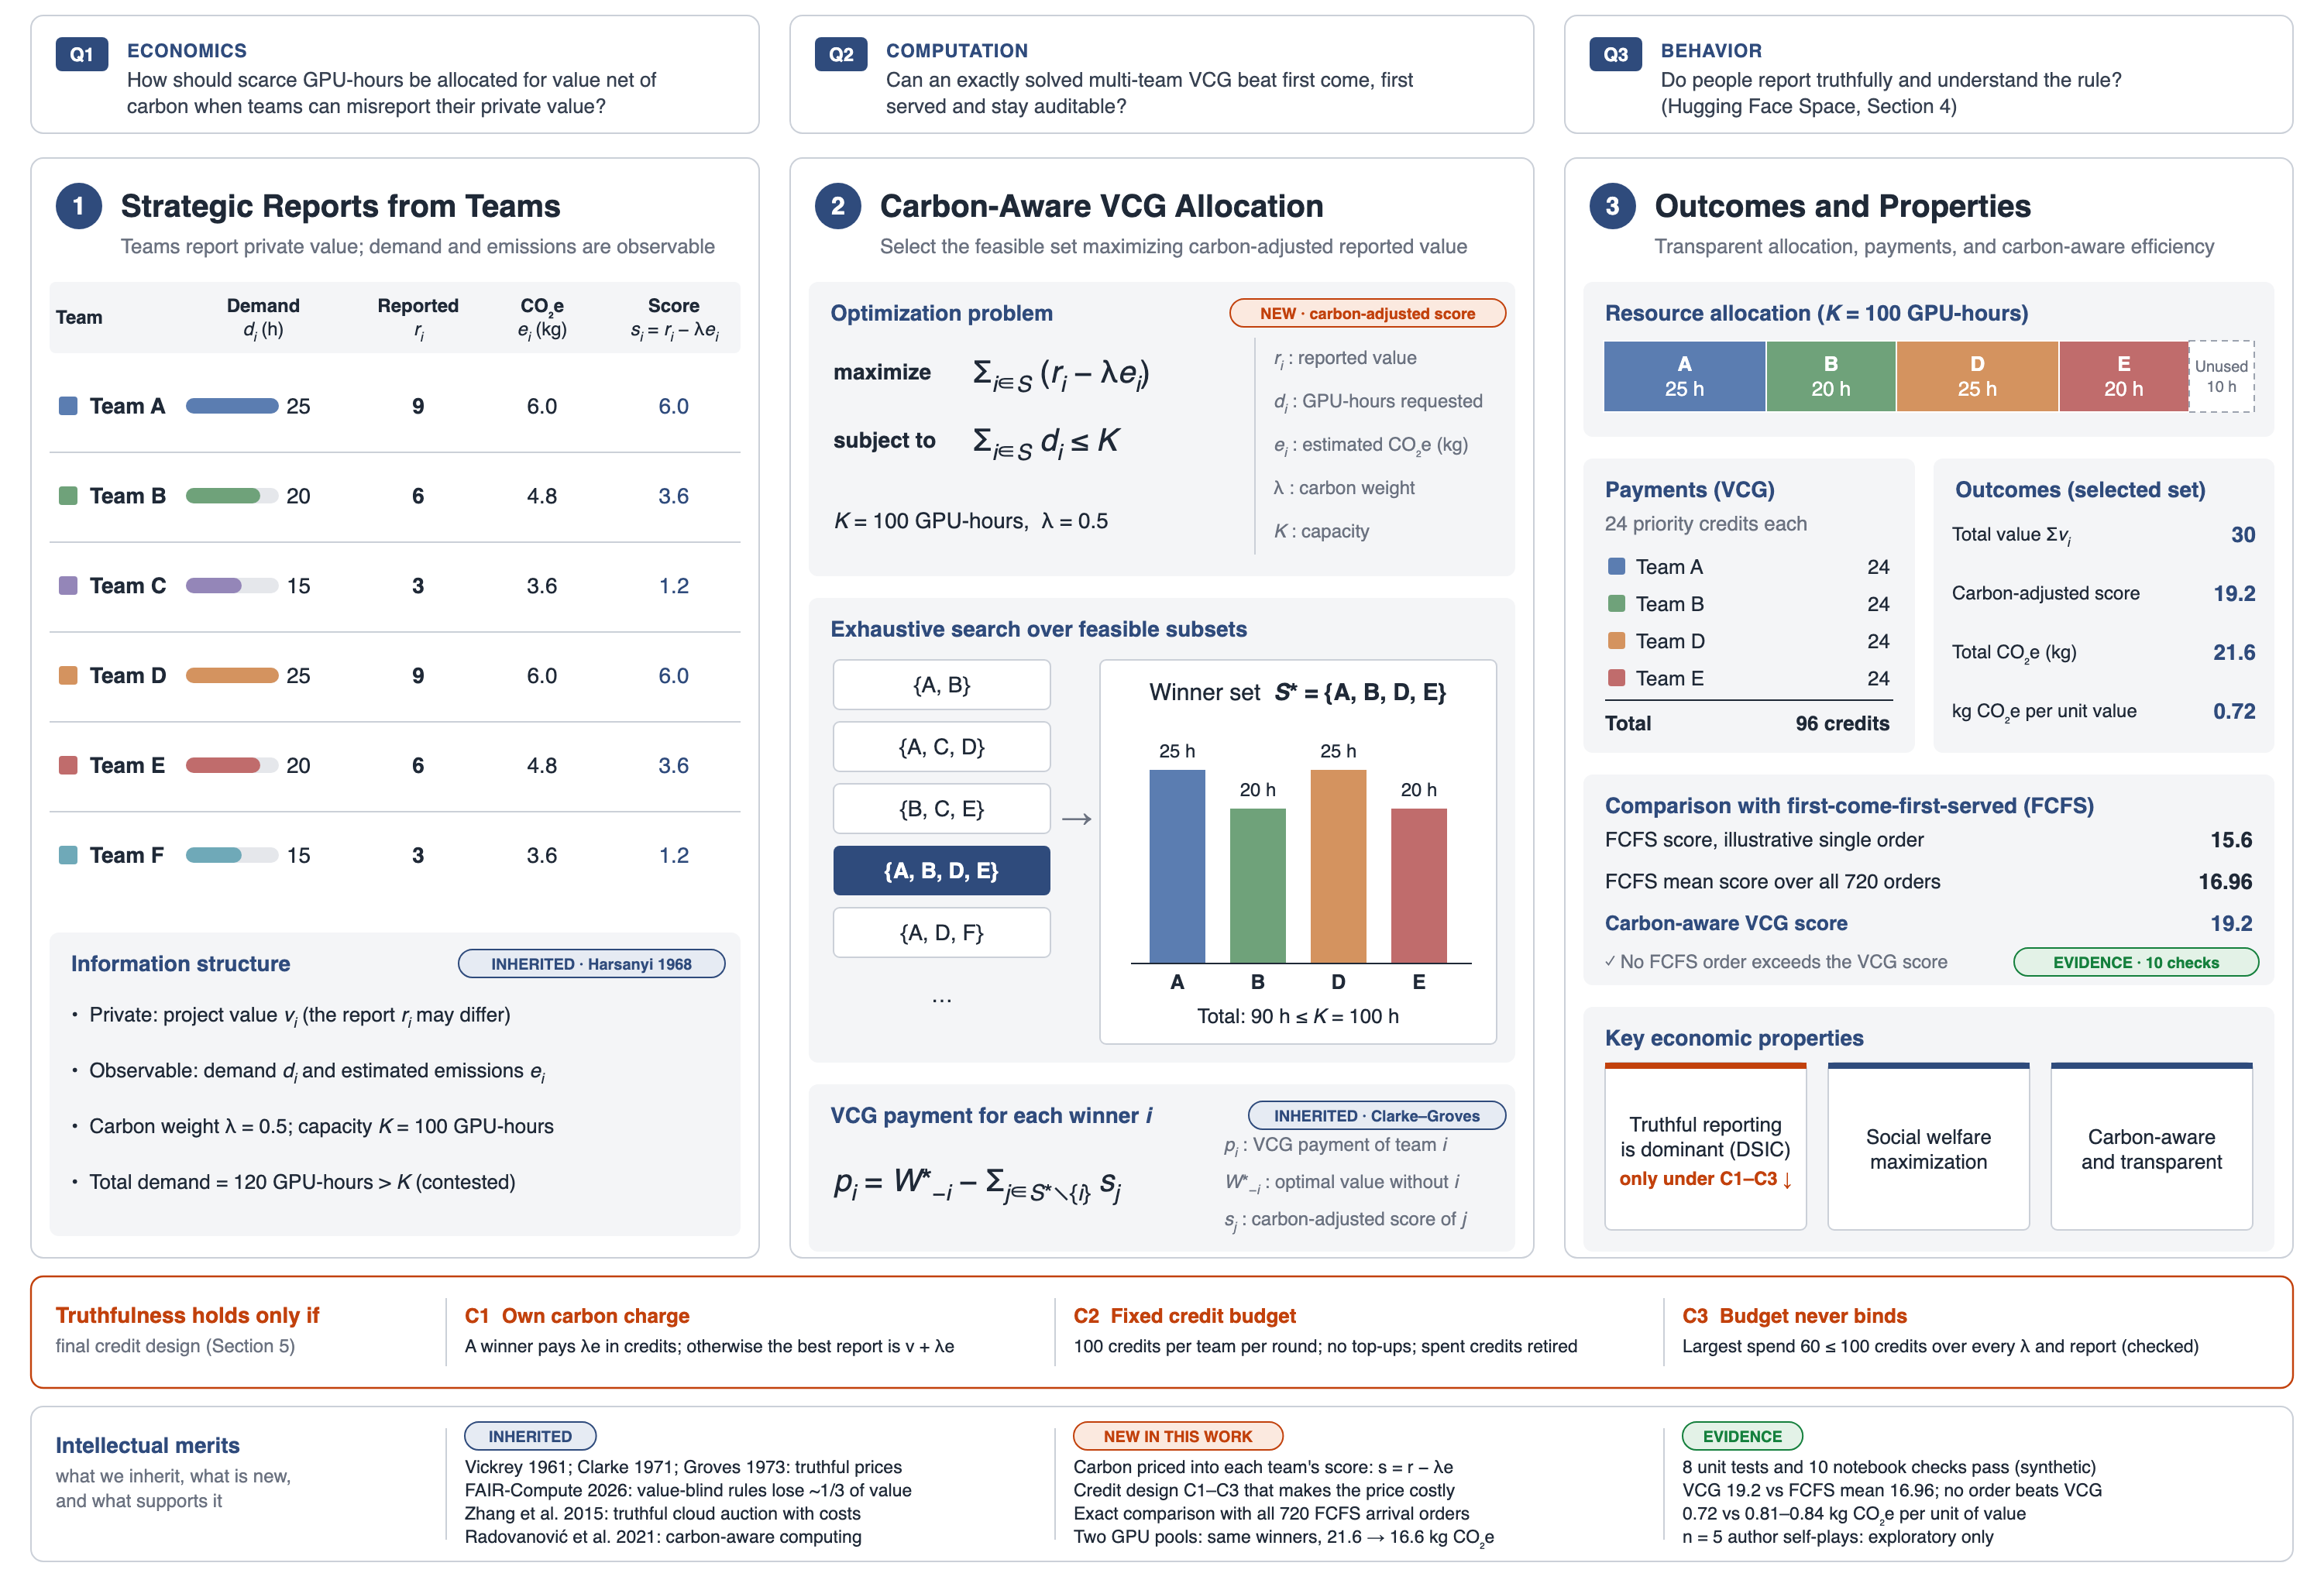
\includegraphics[
  width=\textwidth,
  keepaspectratio
]{figures/teaser_figure.png}
\caption{Carbon-aware GPU-hour allocation: questions, model, exact computation, truthfulness conditions C1--C3 (orange), and merit map: inherited (blue), new (orange), evidence (green). One synthetic instance.}
\label{fig:teaser}
\end{teaserfigure}
\maketitle\raggedbottom\coursemeta

% Two-page main text (final project). The full v2 argument is kept unchanged in Appendix G (appendices/extended.tex).
\providecommand{\needchange}[1]{\textcolor{red}{\textbf{[NEED TO CHANGE: #1]}}}

\section{Background}\label{sec:background}
University GPU clusters still allocate scarce hours mostly by queue. FAIR-Compute replays 20.9 million academic jobs and finds that value-blind rules recover only about 65\% of the available scientific value; it does not quantify carbon and leaves mechanisms that make truthful value reports optimal to future work~\cite{fair_compute2026}. Truthful cloud auctions price a provider's server cost~\cite{zhang2015iaas}, and carbon-aware schedulers shift flexible load to clean hours without prices or reports~\cite{radovanovic2021carbon}. No rule we found combines a carbon objective with incentives for honest reporting.

\section{Motivation}\label{sec:motivation}
Self-declared value will be exaggerated, and carbon the rule ignores is paid by the public. An institution needs an efficient, carbon-aware, auditable rule whose incentives survive the way payments are made.

\section{Application Scenario}\label{sec:scenario}
A university cluster offers $K=100$ GPU-hours to six teams A--F requesting $d=(25,20,15,25,20,15)$ (120 hours in total). Each team privately knows its project value $v_i\in\{3,6,9\}$; requests and emissions $e_i=0.24d_i$ kg CO$_2$e are public, and the institution announces a carbon weight $\lambda=0.5$. All parameters are stated, synthetic assumptions.

\section{Research Question}\label{sec:rq}
Can a published, carbon-aware VCG rule allocate GPU-hours with more value net of carbon than first come, first served (FCFS), while making truthful reporting optimal---and under which payment conditions? It joins economics (incentives), computation (an exact, auditable comparison), and behavior (do people report truthfully?).

\section{Method}\label{sec:method}
\textbf{Game.} Players: the six teams. Strategy: one report $r_i$, submitted simultaneously (static game, incomplete information). Payoff: $u_i=v_i-\lambda e_i-p_i$ if selected, else 0.
\textbf{Rule.} Score $s_i=r_i-\lambda e_i$; select the feasible group $S^*$ maximizing $\sum_{S}s_i$ subject to $\sum_{S}d_i\le K$, by exact search over all 64 groups; each winner pays the Clarke--Groves externality $p_i=W^*_{-i}-\sum_{j\in S^*\setminus\{i\}}s_j$~\cite{clarke1971,groves1973} in priority credits (10 per score unit).
\textbf{Credit design.} \emph{C1:} a winner pays its own carbon charge $\lambda e_i$ in credits (otherwise the best report is $v_i+\lambda e_i$). \emph{C2:} each team holds a fixed budget of 100 credits per round, with no top-ups; spent credits are retired. \emph{C3:} the budget never binds. Under C1--C3 truthful reporting is dominant~\cite{nash1950,harsanyi1968} by the Groves argument (Appendix~A).
\textbf{Three lenses.} Game theory predicts truthful reports; social choice sets the objective, value net of carbon, with two trade-offs: efficiency against access and truthfulness against budget balance~\cite{greenlaffont1977}; mechanism design specifies and tests the rule.
\textbf{Retained PS2 comparison.} Random-order FCFS over all 720 arrival orders. Analogy boundary: only with one slot and $\lambda=0$ is the rule a Vickrey second-price auction~\cite{vickrey1961} (unit-tested); otherwise several teams win under a knapsack constraint and pay in credits, not money.
\textbf{Checks.} Every report in $[0,10]$ for every team at every $\lambda\in\{0,0.1,\dots,1\}$; two GPU pools; the C3 budget. \textbf{Behavior.} Space players report and predict before seeing the outcome.

\section{Results}\label{sec:results}
\emph{Computed, one synthetic instance} (Appendix~A). VCG selects $\{A,B,D,E\}$ with carbon-adjusted score 19.2; FCFS scores 15.6--19.2 over 720 orders (mean 16.96), and no order beats VCG. Emissions per unit of value fall from 0.81--0.84 to 0.72 kg CO$_2$e, but VCG serves 4 teams against an FCFS mean of 4.93. Winners pay 24 credits each (96 in total) and, with the carbon charge, spend 48--54 of 100; the largest spend over every $\lambda$ and report is 60, so C3 holds. No report beats the truth at any $\lambda$; $\lambda$ moves prices, not the best strategy, so it is a policy weight (above 1.25 only two teams are served). Two GPU pools: same winners, 21.6 to 16.6 kg, truth optimal. \emph{Observed, exploratory} ($n=5$ author self-plays): no misreport paid, yet three of five overreported. 8 unit tests and 10 notebook checks pass.

\section{Intellectual Merits}\label{sec:merits}
Figure~\ref{fig:teaser} marks what is inherited (blue), new (orange), and evidence (green). The closest work, FAIR-Compute~\cite{fair_compute2026} measures the loss from value-blind rules at trace scale without incentives or carbon; we trade scale for an exact instance and build the rule it leaves open. Zhang et al.~\cite{zhang2015iaas} prove truthful cloud auctions with a server-cost term and money; we price carbon instead, pay in budgeted credits, and state the conditions C1--C3 credits need. Radovanovi\'c et al.~\cite{radovanovic2021carbon} shift load to clean hours without prices; we obtain a similar placement inside a strategic rule, with fixed carbon rates. The code check showed that utility $v_i-p_i$ rewards overreporting (computation changed the economics); the self-plays showed truth optimal but not typical (behavior qualified it). Bound: one round, one instance, assumed rates.

\section{Practical Impacts}\label{sec:impacts}
Figure~\ref{fig:impact} (Appendix~G) places the official SDG icons on the mechanism~\cite{un_sdg}. \textbf{Target 9.5} (research capability): carbon-adjusted value 16.96 to 19.2. \textbf{Target 9.4} (resource-use efficiency): 0.81--0.84 to 0.72 kg CO$_2$e per unit of value, 0.55 with two pools. Both are \emph{demonstrated only in simulation}. \textbf{Target 13.3} (institutional capacity on mitigation): a published $\lambda$, a fixed credit supply, and a re-runnable log; \emph{intended}, as no institution has adopted the rule. Stakeholders: teams, administrators, the institution, the public. Risks (safeguards): heavy $\lambda$ trades 9.5 for 9.4 (publish $\lambda$ below 1.25); repeated exclusion (history-based credits, planned); credit inflation (C2); unverifiable values (audit log, ex-post pilot).

\subsection{Future Research Roadmap}\label{sec:roadmap}
Figure~\ref{fig:roadmap} (Appendix~G) starts from one limitation: truth is verified for one round of one instance with fixed carbon rates. \emph{Economics} (Khan): do fixed-budget credits keep truth optimal over 10 rounds, and how should $\lambda$ be announced, as the 2026 prize on expectations suggests~\cite{nobel2026}? With DKU research computing and FP8; December 2026. \emph{Computer science} (Akhtamjonov, Lee): GPU types with measured emissions~\cite{radovanovic2021carbon}, an integer program, and history-based credits~\cite{karma2023}; progress: exact match up to 12 teams, no team excluded over 3 rounds; DKU HPC; spring 2027. \emph{Behavioral} (Lee): reason-before-result study, $n\ge30$, separating misunderstanding~\cite{li2017} from a taste for winning~\cite{cooperfang2008}; 2027.

\smallskip
\noindent{\scriptsize\textbf{Artifacts.} \href{https://github.com/dku-comsci-econ206-Autumn2026/FP05-PS2-Team-A}{GitHub} (tested commit \texttt{\TestedCommit}), \href{https://colab.research.google.com/drive/1xYtctTPKXDszHMjdOS7IVz-OByt4edlD}{Colab}, \href{https://huggingface.co/spaces/dku-comsci-econ206-2026/PS2_Team_A}{Hugging Face Space} (commit \texttt{dddebc7}), A0 poster (\texttt{poster/final-poster.pdf}). 2056 statement and full v2 argument: Appendix~G.\par}

\clearpage\nobalance
\section*{Author Notes}
\subsection*{Acknowledgements}
\textbf{Course instructor: Professor Luyao Zhang.} We thank Prof.~Luyao Zhang for the opportunity to carry out PS1 and PS2 and build our research skills, for the COMPSCI/ECON~206 workshops, and for her formal course feedback of October~14, 2026, which set the final revisions (Appendix~D.1). We thank Prof.~Kenneth S. (Ken) Rogerson for advice on each member's PS1, which became the foundation of our PS2 research question, and Han Zhang for a question on our research idea that made us rethink it and state our research question more concretely.

\textbf{Duet partners (FP8).} We thank Zhenning Wang and Qianshuo (Aaron) Wang, who recommended the three papers closest to our research for the October~12 defense through an Ed post, and who challenged us in the October~12 duet and October~14 roundtable to model more GPU types and to test whether priority-credit payments have a real opportunity cost; the second challenge led us to state C1 (own carbon charge) and C2 (assumed linear opportunity cost) explicitly and to add C3 (a payment-feasibility check) (Section~\ref{sec:method}; Appendix~D.3). We also thank them for the Interdisciplinary Mechanism Design Award and for offering to share their simulation benchmark.

\textbf{Reviewers and discussion partners at the September~28 symposium} (formal peer evaluation; Appendix~D.2). Yiqiao Liu (FP10) asked why the carbon weight is 0.5, which led to the carbon-weight sweep. Qianshuo (Aaron) Wang (FP8) asked how an organization would choose the carbon weight in a real setting, which led us to treat it as a policy weight and bound it with the sweep. Zimu Zhou (FP11) pointed out that only one GPU type was modeled, which led to the two-GPU-pool extension. Xinrong Sun (FP9) asked whether truthful reporting is optimal with and without the carbon charge, which led to the payment intuition in Section~2. Yongzhuo Wu (FP1) pointed out the missing play data in the Hugging Face Space, which led us to record five plays. Zijie Wang (FP7) commented on figure clarity and asked whether the gap is grounded in existing research, which led to the vector teaser figure with a research-question row. Muhan Chen (FP12) noted that results come from one fixed instance, which led us to state that limit and the next study more plainly.

\textbf{Field learning and community.} We acknowledge Tencent's Shanghai office for insight into how AI is applied in real-world industry, the Shanghai Science and Technology Museum for showing the human history and significance of science, and the COMPSCI/ECON~206 classroom community for an environment that pushed us to think about novelty.

\textbf{Data, software, and AI.} All inputs are synthetic and stated in Appendix~A. The SDG icons are the official United Nations icons (\url{https://www.un.org/sustainabledevelopment/news/communications-material/}), used without modification. We rely on Python and its standard library, Jupyter and Google Colab, matplotlib, Hugging Face Spaces, and diagrams.net (draw.io). Generative AI assistance is disclosed in Appendix~A.3. The authors remain responsible for the paper and any remaining errors.

\subsection*{Team and individual contributions}

\textbf{Joint contribution.} Our team studies how an organization can allocate scarce shared GPU-hours when teams privately know their project value but GPU demand and estimated emissions are observable. We compare a random-order FCFS baseline, computed over all 720 arrival orders, with a transparent carbon-aware VCG mechanism that selects a feasible group of teams under a 100 GPU-hour capacity limit. Temur supplies the formal model, exact computation, and reproducibility checks; Mustafa develops the social-choice, governance, and real-world-impact argument; Gihun develops the interactive explanation, artifact interface, and poster layout. These parts form one research argument: a stated allocation rule is useful only when its strategic assumptions, computational results, public explanation, and limits can be inspected together. All three members jointly reviewed the final paper and artifacts for consistency.

\textbf{Temur Akhtamjonov.} I designed the six-team GPU-allocation model, implemented the FCFS baseline and the exhaustive VCG solver, and verified the reported allocation, capacity, score, emissions, and payment outputs. My key decision was to model the setting as a multi-winner direct mechanism rather than a one-winner auction. My evidence is the GitHub simulation, runnable Colab notebook, and saved output files. This work provides the formal and computational basis for the paper, Hugging Face interaction, and poster. Before the symposium, my responsibility was to check that all three artifacts use the same parameters, allocation rule, and reported results. After the symposium, I verified that the carbon-weight sweep and two-GPU-pool extension preserve capacity feasibility and the truthful-reporting benchmark in the final rerun (seven unit tests and nine notebook checks). My next responsibility is to rerun the FCFS--VCG comparison over randomly drawn values and requests (Appendix~D) and to keep the paper, code, Space, and poster aligned with the final parameters.

\textbf{Mustafa Ayub Khan.} I developed the social-choice and mechanism-design framing: writing the literature review identifying FAIR-Compute as the closest prior work and the specific gap it leaves open---an incentive-compatible, carbon-aware allocation rule it names as future work but does not build---and drafting the real-world-impact case distinguishing academic, industry, and public-institution evidence standards for adoption. My key decision was identifying that an early fixed-price allocation formula (score proportional to GPU-hours alone) had silently dropped private project value from the mechanism, and proposing the corrected selection rule $s_i = r_i - \lambda e_i$, which restores private value as the basis for selection and keeps demand as only a capacity constraint---the formula the team's VCG mechanism is built on. I also treated auditability of execution, not verification of private values, as the honest limit of this mechanism's transparency. My evidence is Sections~1, 2, and~5, the Open Science and SDG statements, and Table~1's roadmap. I independently re-derived Temur's FCFS and VCG allocation numbers by hand against the stated $v_i$, $d_i$, and $\lambda=0.5$, confirming the reported subsets, scores, and total payment of 9.6 score units (96 priority credits). This argument depends on Temur's simulation producing the value/carbon trade-off Section~5 describes, and feeds the poster's real-world-case panel and Gihun's audit-trail framing in the Hugging Face interface. Before the symposium, my responsibility was to check symposium feedback against Section~5's adoption-evidence claims. After the symposium I kept the existing-research comparison (Zijie Wang), since the FAIR-Compute comparison was already verified, and logged the single synthetic instance (Muhan Chen) and the real-world value of $\lambda$ (Qianshuo (Aaron) Wang) as open Investigate items in Appendix~D; the carbon-intensity concern (Zimu Zhou) is now addressed by the two-pool extension. My next responsibility is to investigate realistic carbon-intensity values by GPU type and an institutional carbon price to ground $\lambda$, then revise the real-world case in Section~5.

\textbf{Gihun Lee.} I built the public-facing allocation audit and the reproducibility interface: the Hugging Face Space, the GitHub README, the self-contained Colab notebook structure, Figure~\ref{fig:teaser}, and the poster layout. My key decision was to make the stated rule checkable against its visible execution: in the Space a player holds a private true value, reports separately, predicts their own selection, and then sees the score ranking, winning group, VCG payments, utility, and a what-if curve of utility against every report. While building this audit, I found that the original utility $v_i-p_i$ contradicted the paper's dominant-strategy claim, because under it a team gains by reporting $v_i+\lambda e_i$. I proposed $u_i=v_i-\lambda e_i-p_i$, added a truthfulness sweep, and replaced the single FCFS queue with all 720 arrival orders. My evidence is the Space, the \texttt{colab/} folder (tests, outputs, notebook), and the README. I verified that the unit tests pass, that the notebook runs 9/9 checks in a clean folder without the repository, that the browser port reproduces the repository outputs for the fixed example and passes a truthfulness check on 200 random instances (\texttt{node hf-space/app.js}), and that \texttt{run\_simulation.py} reproduces the committed outputs. This work turns Temur's computation and Mustafa's framing into an interface a non-specialist can inspect. \emph{Revision after the symposium.} I recorded six peer reviews of the project on my response form and made the following revisions (decisions in Appendix~D, change list in Appendix~F.3).
(1)~\emph{Carbon weight} (Yiqiao Liu, Qianshuo (Aaron) Wang): I swept $\lambda$ from 0 to 1 and reported both what it changes (prices, payoffs, selection boundaries) and what it cannot change (the best strategy). My key decision was to treat $\lambda$ as a policy weight rather than a parameter to optimize, because on project value alone $\lambda=0$ always wins. Output: the notebook's sweep cells, \texttt{run\_simulation.py}, and \texttt{lambda\_sweep.csv}; Section~3 and Appendix~A.2.
(2)~\emph{GPU types} (Zimu Zhou): I added a two-pool extension (H100 and A100) in which the rule also chooses each team's pool, and recorded its limit, that it ignores speed differences. Output: notebook, Appendix~A.2--A.3.
(3)~\emph{Truthfulness with and without the carbon charge} (Xinrong Sun): I added the payment intuition to Section~2 and the exact selection boundary for Team C ($r_C\ge4.2$), and I stated the analogy boundary in Section~3 with a unit test showing that one slot with $\lambda=0$ is a second-price auction.
(4)~\emph{Missing play data} (Yongzhuo Wu): I added the behavioral mechanism, the competing explanation, and the computed consequence of each behavior type to Section~4. My key decision here was to label these rows as computed and to report the five recorded plays separately as observed, so that simulated behavior is never presented as observed behavior.
(5)~\emph{Figure clarity} (Zijie Wang): I re-exported Figure~\ref{fig:teaser} as a vector PDF and added a top row that states the three research questions, so the figure itself shows how Q1--Q3 connect to the panels. Output: \texttt{figures/teaser\_figure.pdf}, \texttt{.svg}, \texttt{.png}, and the editable \texttt{.drawio}.
(6)~\emph{Other revisions}: the method-by-method comparison with the closest work in Section~1, the budget-balance trade-off in Section~2 and Appendix~C, the corrected $\lambda$ statement in Appendix~C, the README, and Appendices~D, E, and F.3. My next responsibility is to collect more plays with the written reflection filled in, show the what-if curve before the report, and keep the poster, paper, and artifacts at parity.

\textbf{Final-week contributions (October~12--21, 2026).} Each author owned one response to the final-week challenges; decisions are recorded in Appendix~D.
\emph{Mustafa Ayub Khan} raised the self-challenge that truthfulness fails if credits cost nothing, and owns the resulting credit design (C1: own carbon charge; C2: a stated linear opportunity-cost assumption; C3: a fixed per-round budget with no top-ups and retired credits, used to check payment feasibility), the Practical Impacts section and diagram (Section~\ref{sec:impacts}, Figure~\ref{fig:impact}), and the economics study in the roadmap; he is responsible for checking names and contributions in the paper and poster.
\emph{Temur Akhtamjonov} raised the self-challenge that one GPU type limits real use, kept the two-pool result as a structural check, and owns the extension to several GPU types with measured emissions in the computer-science study; he is responsible for verifying that the symposium and final-week revisions are reflected in all artifacts.
\emph{Gihun Lee} raised the self-challenge that the same low-value teams may lose every round and that choosing $\lambda$ is political. He implemented and checked the budget condition C3 (notebook cell and unit test; 8 tests and 10 notebook checks pass), annotated Figure~\ref{fig:teaser} with the incentive conditions and the inherited/new/evidence map, built the roadmap (Section~\ref{sec:roadmap}, Figure~\ref{fig:roadmap}), compressed the main text to two pages, compiled Appendix~D, and owns the history-based-credit and behavioral studies.

\bibliographystyle{ACM-Reference-Format}\bibliography{references}
\appendix
\section{Technical details and reproducibility}

\subsection{Model inputs and rules}

This project uses one fixed synthetic classroom example with six teams and a capacity of $K=100$ GPU-hours. Table~\ref{tab:inputs} gives the inputs. Values are private to teams but are reported truthfully in the baseline computation. GPU-hour demand is observable. Estimated emissions use the stated classroom assumption $e_i=0.24d_i$ kg CO$_2$e. The announced carbon weight is $\lambda=0.5$, so each reported score is
\[
s_i=r_i-\lambda e_i=r_i-0.5(0.24d_i).
\]

\begin{table}[h]
\centering
\caption{Fixed synthetic inputs used in the fresh run.}
\label{tab:inputs}
\begin{tabular}{lrrr}
\toprule
Team & GPU-hours $d_i$ & Value $v_i$ & Emissions $e_i$ \\
\midrule
A & 25 & 9 & 6.0 \\
B & 20 & 6 & 4.8 \\
C & 15 & 3 & 3.6 \\
D & 25 & 9 & 6.0 \\
E & 20 & 6 & 4.8 \\
F & 15 & 3 & 3.6 \\
\bottomrule
\end{tabular}
\end{table}

The FCFS baseline uses a random arrival order. Each team receives its full request only when the request fits in the remaining capacity. We compute all $6!=720$ orders exactly and report A, B, E, C, D, F as one illustrative draw. The proposed mechanism is a simultaneous-report, multi-winner VCG direct mechanism. It chooses the feasible subset $S$ that maximizes total reported score:
\[
\max_{S \subseteq N}\sum_{i\in S}s_i
\quad \text{subject to} \quad
\sum_{i\in S}d_i\leq K.
\]
For each selected team $i$, the priority-credit payment is its reported-score externality:
\[
p_i=
\max_{S'\subseteq N\setminus\{i\}}\sum_{j\in S'}s_j
-
\sum_{j\in S\setminus\{i\}}s_j.
\]
One payment score unit equals 10 non-transferable priority credits in this classroom model. A selected team's utility is \ensuremath{u_i=v_i-\lambda e_i-p_i}, and an unselected team's utility is \ensuremath{0}. \textbf{Credit design (final version).} C1: a selected team pays its own carbon charge \ensuremath{\lambda e_i} in credits. C2: the model assumes that a credit charged to a team has a linear opportunity cost, as represented by the stated utility. C3: each team has a fixed budget of 100 credits per allocation round, with no top-ups, and spent credits are retired; the budget does not bind in the tested cases. Under C1 and the C2 utility assumption, truthful reporting is dominant by the Groves argument. C3 establishes payment feasibility only; it does not prove that credits have real opportunity cost. At \ensuremath{\lambda=0.5}, A and D spend \ensuremath{30+24=54} credits and B and E spend \ensuremath{24+24=48} credits; over every tested carbon weight and report with rivals truthful, the largest spend is 60 credits, below the budget (notebook cell ``Credit budget''; unit test \texttt{test\_round\_budget\_never\_binds}).

\textbf{Reduced payoff matrix.} The full game has six players and a continuum of reports, so it has no single matrix. Table~\ref{tab:matrix} is a labeled simplification: only Teams C and E choose, each between its truthful report and one deviation, while A, B, D, and F report truthfully. Every cell is computed by the same \texttt{vcg\_allocation} code (notebook cell ``Reduced payoff matrix'').

\begin{table}[h]
\centering
\caption{Reduced $2\times2$ game: utilities $(u_C,u_E)$ and the selected group.}
\label{tab:matrix}
\footnotesize
\begin{tabular}{lcc}
\toprule
 & E truthful ($r_E=6$) & E underreports ($r_E=4$) \\
\midrule
C truthful ($r_C=3$) & $(0,\;1.2)$, ABDE & $(0.8,\;0)$, ABCDF \\
C overreports ($r_C=4.5$) & $(-1.2,\;0)$, ABCDF & $(0.8,\;0)$, ABCDF \\
\bottomrule
\end{tabular}
\end{table}

For Team C, the truthful row is never worse than the overreport row ($0\ge-1.2$ and $0.8\ge0.8$). For Team E, the truthful column is never worse than the underreport column ($1.2\ge0$ and $0\ge0$). Truth is therefore weakly dominant for both, and (truthful, truthful) is the equilibrium of the reduced game, matching the dominant-strategy result of the full model. The lower-left cell also shows the externality: C's overreport removes the truthful Team E from the group.

\subsection{Exact algorithm and fresh-run record}

The implementation checks every possible subset of six teams.

\begin{enumerate}
\item Enumerate all $2^6=64$ subsets.
\item Remove a subset if its total requested GPU-hours exceed 100.
\item Compute total reported score for every remaining subset.
\item Select the subset with the largest score. Ties are broken publicly by first serving more teams and then using deterministic team order.
\item For each selected team, repeat the calculation without that team and compute its externality payment.
\item Truthfulness check: for each team, re-run steps 1--5 with its report set to $0,0.5,\dots,10$, holding the other teams fixed, and confirm that no report beats $r_i=v_i$.
\item Carbon-weight sweep: repeat steps 1--6 for $\lambda=0,0.1,\dots,1$.
\item Two-GPU-pool extension: choose who is served and on which pool (all $3^6=729$ assignments), then repeat steps 5--6.
\item Credit-budget check (C3): over steps 6--7, record each selected team's spend $10(\lambda e_i+p_i)$ and confirm that it never exceeds the 100-credit budget.
\end{enumerate}

A fresh run of \texttt{python colab/run\_simulation.py} reproduces the saved summary, team-level, all-orders, truthfulness, and carbon-weight-sweep CSV outputs in the repository's \texttt{colab/outputs} folder. The same calculation is available in our self-contained Colab notebook (\NotebookLink).

The saved fresh-run comparison is:

\begin{center}
\small\setlength{\tabcolsep}{3pt}
\begin{tabularx}{\columnwidth}{@{}Yrrrr@{}}
\toprule
Rule & GPU-h & Value & CO$_2$e & Score \\
\midrule
FCFS (A,B,E,C,D,F) & 95 & 27 & 22.8 & 15.6 \\
FCFS, 720-order mean & 97.0 & 28.6 & 23.28 & 16.96 \\
VCG (A,B,D,E) & 90 & 30 & 21.6 & 19.2 \\
\bottomrule
\end{tabularx}
\end{center}

In the illustrative order, FCFS serves A, B, E, C, and F and leaves 5 GPU-hours unused. Across all 720 orders, the FCFS carbon-adjusted score ranges from 15.6 to 19.2, and no order exceeds VCG. VCG leaves 10 GPU-hours unused and collects 9.6 payment score units, equal to 96 priority credits (2.4 per winner). Utilities are 3.6 for A and D, 1.2 for B and E, and 0 for C and F. For every team, no tested report on the grid $\{0,0.5,\dots,10\}$ yields higher utility than $r_i=v_i$. The notebook's final cell prints PASS for ten checks: allocation, capacity, value and score, payments, utilities, truthful optimality, the 720-order comparison, truthful optimality at every carbon weight, the two-GPU-pool extension, and the credit budget (C3). A repository test confirms that the notebook's model code is identical to \texttt{colab/src/gpu\_allocation.py}.

\textbf{Carbon-weight sweep} (\texttt{colab/outputs/lambda\_sweep.csv}; demands, values, capacity, and algorithm fixed).

\begin{center}
\footnotesize\setlength{\tabcolsep}{3pt}
\begin{tabularx}{\columnwidth}{@{}rYrrrc@{}}
\toprule
$\lambda$ & Selected & Pay & $u_{A,D}$ & $u_{B,E}$ & Truth \\
\midrule
0.0 & A,B,C,D,F & 6.0$^{*}$ & 3.00 & 0.00 & yes \\
0.1 & A,B,D,E & 5.28 & 3.12 & 0.24 & yes \\
0.3 & A,B,D,E & 3.84 & 3.36 & 0.72 & yes \\
0.5 & A,B,D,E & 2.40 & 3.60 & 1.20 & yes \\
0.7 & A,B,D,E & 0.96 & 3.84 & 1.68 & yes \\
0.9 & A,B,D,E & 0.00 & 3.60 & 1.68 & yes \\
1.0 & A,B,D,E & 0.00 & 3.00 & 1.20 & yes \\
\bottomrule
\end{tabularx}
\end{center}
{\footnotesize Pay: payment per winner in score units. $^{*}$At $\lambda=0$, C and F pay 3.0. Truth: no report in $[0,10]$ beats $r_i=v_i$ for any team. The CSV holds all eleven values.}

\emph{What $\lambda$ changes.} It moves each team's selection boundary, the price, and the size of the payoff. At low $\lambda$ the low-value teams C and F still compete for a seat, so winners pay more (5.28 at $\lambda=0.1$). As $\lambda$ rises their scores turn negative, competition fades, and the price falls to 0 from $\lambda=0.9$; from that point a heavier own carbon charge $\lambda e_i$ lowers the winners' utility. Team C's selection boundary moves from $r_C\ge3.25$ ($\lambda=0.1$) to 4.2 ($\lambda=0.5$) and 4.8 ($\lambda=1$).
\emph{What $\lambda$ does not change.} Truthful reporting is optimal for every team at every $\lambda$ in the sweep, because a team's price never depends on its own report. $\lambda$ is a policy weight on carbon, not an incentive parameter. It also cannot be chosen by maximizing project value: on value alone, $\lambda=0$ always wins.
\emph{The change at $\lambda=0$.} Groups $\{A,B,C,D,F\}$ and $\{A,B,D,E\}$ tie on value (30). The public tie-break selects more teams; any $\lambda>0$ breaks the tie toward the group that uses fewer GPU-hours.
\emph{Beyond the tested sweep.} In this synthetic instance, above $\lambda=1.25$ only A and D are served, and above $\lambda=1.5$ no team is served. These thresholds depend on the chosen values, demands, emissions rate, and tie-break; they are not general policy cutoffs.

\textbf{Two-GPU-pool extension} (notebook only). The 100 GPU-hours are split into an H100 pool (50 h, 0.24 kg CO$_2$e per GPU-hour, the baseline rate) and an A100 pool (50 h, 0.14 kg). A team runs entirely on one pool, and the score uses the assigned pool's rate.

\begin{center}
\footnotesize\setlength{\tabcolsep}{3pt}
\begin{tabularx}{\columnwidth}{@{}p{2.3cm}YY@{}}
\toprule
 & One pool & Two pools \\
\midrule
Selected & A, B, D, E & A, B, D, E \\
Placement & --- & A, D on A100; B, E on H100 \\
CO$_2$e (kg) & 21.6 & 16.6 ($-23\%$) \\
kg per unit value & 0.72 & 0.55 \\
Payments & 2.4 each & A, D 3.65; B, E 2.4 \\
Utilities & A, D 3.6; B, E 1.2 & unchanged \\
Truth optimal & yes & yes \\
\bottomrule
\end{tabularx}
\end{center}

The two largest jobs move to the cleaner pool. A and D pay more because, without A, other teams could use its clean A100 hours, so A's externality is larger. Utilities and selection boundaries are unchanged, and no report beats the truth: the Groves argument needs only that the best feasible outcome is found exactly, however many capacity constraints there are.

\subsection{Reproducibility, limits, and AI-use disclosure}

\textbf{Reproducibility.} The GitHub repository (\GitHubLink) contains the source code, tests, notebook, output files, and README instructions in \texttt{colab/}. The model, script, and tests use only the Python standard library. The notebook's utility plots use matplotlib, which Colab provides. Review-ready results come from commit \texttt{d93fc2e}; PS2 final results (v2) come from commit \texttt{8a656a4} on the \texttt{main} branch of the classroom repository. Rerun, October 3, 2026 (Python 3.14.7, macOS arm64): \texttt{run\_simulation.py} reproduces the committed outputs and writes \texttt{lambda\_sweep.csv}; 7 unit tests pass; the notebook passes 9/9 checks in an empty folder without the repository. Final rerun, October~17, 2026, after adding the credit budget: outputs reproduced without a diff, 8 unit tests pass, and the notebook passes 10/10 checks; tested commit \texttt{\TestedCommit} (Appendix~D.8).

\textbf{Limits.} This is a small synthetic example, not a field deployment. The 0.24 kg CO$_2$e per GPU-hour rate, the carbon weight, the value tiers, and the 10-credit conversion are classroom assumptions. Exact enumeration will not remain practical as the number of teams becomes large. The model also cannot verify a team's true private value. The baseline has one GPU type; the two-pool extension assumes a job needs the same GPU-hours on either type, whereas an A100 is slower than an H100 in practice, so it is a structural check and not an emissions estimate. Truthful reporting is dominant only under C1 and the C2 linear-opportunity-cost assumption; the code checks that the 100-credit budget does not bind in this instance, but does not establish that teams value credits across repeated rounds. Human play is limited to five self-plays by the authors against simulated, truthful rivals with hypothetical stakes, and their written reflections are blank.

\textbf{AI-use disclosure.} The team used Claude Code (Claude Opus 5.5, Anthropic) from \emph{September~25 to October~19, 2026}.
\emph{Purpose:} build the Hugging Face Space, jupyter notebook, the simulation code, and the unit tests; respond to the September~28 symposium reviews and to the October~12--14 feedback; and prepare the final release (paper, figures, poster, and README).
\emph{Significant prompts:} sweep $\lambda$ from 0 to 1; simulate two GPU types; add a credit-budget check; check the draft against the grading guide and the scoring card; annotate Figure~\ref{fig:teaser}; draft the impact and roadmap diagrams, Appendix~D, and the acknowledgments from the team's own notes; compress the main text to two pages; update the poster.
\emph{Accepted:} the simulation code, the unit tests (including the C3 budget test), the carbon-weight sweep, the two-GPU-pool cells, the reduced payoff matrix, the Figure~\ref{fig:teaser} research-question row and annotations, the two new diagrams, and drafts of the main text and Appendices~A and D--G. \emph{Rejected:} full redesigns of Figure~\ref{fig:teaser}.
\emph{Human decisions:} the research question and the model; the credit design (C1--C3), chosen by the team at the roundtable; the SDG targets, chosen by the authors from the official list; the wording of every section, revised by the authors.
\emph{Checks:} unit tests, fresh notebook runs, the Space self-check (\texttt{node hf-space/app.js}), a fresh compile of the Overleaf source, and source checks of every new citation (Crossref, arXiv, USENIX, the Royal Swedish Academy of Sciences).

\section{Cumulative Intellectual Development}
\textbf{Mustafa Ayub Khan -- prior development.} In PS1, Mustafa studied whether greater observability changes voluntary disclosure in a public-goods setting. Following Professor Zhang's September 7 feedback, he narrowed the claim and proposed a 2-by-2 design to distinguish genuine behavioral change from merely visible performance. This led to one bounded lesson for PS2: making a rule and its execution observable can improve accountability, but it cannot prove that a participant's private motive or value report is true. In the GPU-allocation project, this lesson appears in the published allocation rule, parameters, code, payments, and allocation log.

\textbf{Gihun Lee -- prior development.} In PS1, Gihun developed a transparent way to compare heterogeneous AI subscription plans using workload-specific measures, reproducible computation, sensitivity checks, and a public-facing interaction. Feedback on trustworthiness led him to avoid one opaque summary number and instead show the underlying components and assumptions. In PS2, this becomes the Hugging Face allocation audit: users can compare FCFS and the VCG mechanism, inspect the reported inputs and outcomes, see the stated assumptions behind the result, and check with a what-if curve whether truthful reporting maximizes their own utility. The same lesson shaped the revision after the September 28 symposium: reviewers asked why $\lambda=0.5$ and whether one GPU type is enough, so instead of defending one headline number Gihun showed the components. The carbon-weight sweep reports what $\lambda$ changes (prices, payoffs, selection boundaries) and what it does not (the best strategy); the two-GPU-pool extension reports which results survive a second capacity constraint; and Figure~\ref{fig:teaser} now states the three research questions above the panels. Affected locations: Sections~2--4, Appendix~A.2, and Figure~\ref{fig:teaser}.

\textbf{Temur Akhtamjonov -- development into the shared model.} Temur's earlier work on a commitment-bond trust game used a clear benchmark, a controlled rule change, and verified computational outputs. In PS2, he transfers this methodological approach to a new shared setting: hold the six-team GPU environment fixed, compare FCFS with carbon-aware VCG, enumerate all feasible allocations exactly, and report the resulting allocation and payments.

\textbf{Intellectual consequence.} PS2 is a new joint project, not a continuation of one PS1 topic. Its common development is methodological: each prior project emphasized a clear rule, visible assumptions, reproducible computation, and careful limits on what observed behavior can establish. Our shared contribution applies these principles to a transparent, carbon-aware allocation of scarce organizational GPU-hours.

\section{Open-source and three-lens inspiration}
\textbf{Sources and tools.} PS1 source records are preserved in each author's PS1 submission; the tools below are those used in PS2.

{\footnotesize
\begin{tabularx}{\columnwidth}{@{}p{1.6cm}Y@{}}\toprule
\textbf{Source / tool}&\textbf{URL, license, version; capability; limitation; design consequence}\\\midrule
Python standard library&\url{https://www.python.org}; PSF License; 3.13--3.14 locally, Colab runtime. Exact subset enumeration and permutations with no installs. Exponential in team count. Kept the model dependency-free so anyone can re-run it.\\
Jupyter / Google Colab&\url{https://jupyter.org} (BSD-3), \url{https://colab.research.google.com} (Google service terms). Runnable notebook with saved outputs. Hosted runtime can change over time. Notebook made self-contained, with a test that it matches \texttt{src/}.\\
matplotlib&\url{https://matplotlib.org}; matplotlib license (PSF-based); 3.11. Utility-versus-report plots. Plots only. Used only outside the model code.\\
Hugging Face Spaces (static)&\url{https://huggingface.co/docs/hub/spaces-sdks-static}; hosted service. Serves an HTML/CSS/JS page with no server. Cannot store responses. Evidence is collected by participants copying a result line rather than by server logging.\\
Claude Code&\url{https://claude.com/claude-code}; Anthropic terms; Claude Opus 5.5, Sept.--Oct.~2026. Coding and drafting assistant. Can err, so all outputs were tested. See Appendix~A.3.\\\bottomrule
\end{tabularx}}

\textbf{How each lens altered the shared model.}
\emph{Game theory:} framing the setting as a static game with incomplete information made $r_i=v_i$ the benchmark to test. Testing it (observation) showed that the original utility $v_i-p_i$ rewards overreporting by $\lambda e_i$, so the utility now includes each team's own carbon penalty.
\emph{Social choice:} stating the objective as value net of carbon under capacity exposed the efficiency--access trade-off. VCG serves 4 teams against an FCFS mean of 4.93 (observation). We interpret this as a real cost of the rule rather than a flaw to hide. A second incompatibility is budget balance: the 96 credits collected go to the organization, not back to the teams, because redistributing them would in general break truthfulness~\cite{greenlaffont1977}.
\emph{Mechanism design:} it fixed the report space, allocation, payment, and public tie-break, and it turned FCFS from one arbitrary queue into all 720 orders. The $\lambda$ sweep (observation) shows that the winning group is the same for every $\lambda\in[0.1,1]$ and differs only at $\lambda=0$, where two groups tie on value and the public tie-break decides; payoffs change with $\lambda$, but truthful reporting stays optimal throughout. A two-GPU-pool extension (observation) leaves the winners and the incentives unchanged while moving the largest jobs to the cleaner pool.
All three results are computed from the formal model. Whether people report truthfully is observed only in five exploratory plays (Section~4); a larger classroom sample remains planned.

\clearpage
\onecolumn
\section{Review response and revision record}
\textbf{Status.} This is the final version (v3, October~21, 2026). The review-ready version (v1, September~27) is preserved at commit \texttt{d93fc2e} and the PS2 final version (v2) at commit \texttt{8a656a4}. Each consequential comment receives a Keep (K), Revise (R), or Investigate (I) decision, the changed location, the verification or next test, and the responsible author. Earlier records are preserved below; nothing was removed.

\subsection{Instructor feedback on PS2 (October~14, 2026)}
The PS2 score (19.5/20) is unchanged; these items guide the final project. We preserve the strengths the feedback named: the consistent allocation objective, payments, and carbon-adjusted utility in Section~2, and the exact comparison with all 720 FCFS orders.

\medskip
\noindent{\footnotesize
\begin{tabularx}{\textwidth}{@{}p{0.13\textwidth}p{0.17\textwidth}Yp{0.075\textwidth}@{}}
\toprule
\textbf{Source and date} & \textbf{Affected claim} & \textbf{Decision, change, location, and verification} & \textbf{Owner} \\
\midrule
Prof.~Luyao Zhang, formal feedback, Oct.~14 & Truthfulness claim in Figure~1 and the poster: each user must bear the carbon charge, and credits need a real opportunity cost & \textbf{R.} C1 (own carbon charge) and the C2 linear-opportunity-cost assumption now stand beside the claim: Section~\ref{sec:method} (``Credit design''), the orange strip and DSIC box of Figure~\ref{fig:teaser}, Appendix~A.1. C3 is checked for payment feasibility: largest spend 60 of 100 credits over every $\lambda$ and report (notebook cell ``Credit budget''; \texttt{test\_round\_budget\_never\_binds}). Poster (final v3): C1 and C2 beside the claim in the strategic-model panel, C3 labeled as a feasibility check. & Mustafa (design), Gihun (figure, check) \\
 & Main argument runs to page~4 & \textbf{R.} Done: the main text is now two pages with the eight named parts and a Future Research Roadmap subsection; the full v2 Sections~1--5 are kept unchanged in Appendix~G, and extended sweeps stay in Appendix~A. & All \\
 & Five self-plays in Appendix~F.1 have blank reflections & \textbf{K} (records). The five records are preserved unchanged with the missing-reflection limitation; no reasons were reconstructed. \textbf{R} (protocol): new plays must record a written reason before the result is shown (roadmap, behavioral study). & Gihun \\
 & SDG 9 and 13 claims need measured emissions and a real credit cost & \textbf{R.} Targets 9.5, 9.4, and 13.3 with official icons (Figure~\ref{fig:impact}); 9.5 and 9.4 labeled demonstrated in simulation only, 13.3 intended. Credit cost: stated as the C2 assumption, with C3 checking feasibility. \textbf{I.} Measured emissions: computer-science study (Figure~\ref{fig:roadmap}). & Mustafa, Temur \\
 & Compare three closest papers; invite the partner to challenge who pays for emissions and credits & \textbf{R.} Sections~\ref{sec:background} and~\ref{sec:merits} now compare FAIR-Compute, Zhang et al.~(2015), and Radovanovi\'c et al.~(2021) by method, assumption, and evidence; Figure~\ref{fig:teaser} marks them as inherited. The partner's credit challenge is in D.3. & Mustafa, Gihun \\
 & Defend one carbon-weight adverse case and name evidence that would reverse the design & \textbf{K} with a stated reversal test. Adverse case: in this synthetic instance, above $\lambda=1.25$ only A and D are served, and above $\lambda=1.5$ no team is served. The model does not justify a general cap. A real institutional value of $\lambda$ requires local carbon-price and operational data. Reversal: if such data imply a materially different carbon trade-off, or if ex-post outcomes show that excluded compute-heavy projects had higher realized value than the winners, we would revise the design, for example by using a carbon-budget constraint instead of this price. & Gihun \\
\bottomrule
\end{tabularx}}

\subsection{Peer reviews at the September~28 symposium}
Each author recorded the reviews on an individual response form. \emph{By} names the forms that recorded each comment (G: Gihun Lee; M: Mustafa Ayub Khan; T: Temur Akhtamjonov).

\noindent{\footnotesize
\begin{tabularx}{\textwidth}{@{}p{0.10\textwidth}p{0.15\textwidth}p{0.045\textwidth}Yp{0.065\textwidth}@{}}
\toprule
\textbf{Reviewer} & \textbf{Key point} & \textbf{By} & \textbf{Decision, change, and verification} & \textbf{Owner} \\
\midrule
Yongzhuo Wu (FP1) & No actual player data in the Hugging Face Space. & G, T & \textbf{I}, then \textbf{R.} Correct at the symposium: no plays had been collected. We have since recorded $n=5$ completed self-plays by the three authors (October~3, 2026) and exported them (\texttt{hf-space/plays.csv}). Result: no misreport raised utility, but three of five players overreported and the reflections are blank. We also added the computed consequence of each behavior type, labeled as computed. A larger sample with reflections remains planned. Location: Section~4, Appendix~F.1. & Gihun \\
Zimu Zhou (FP11) & Only one GPU type, with one carbon intensity, is modeled. & G, M, T & \textbf{R.} Added a two-pool extension (H100 50\,h at 0.24\,kg; A100 50\,h at 0.14\,kg). Rerun: the same four teams win, A and D are placed on A100, emissions fall from 21.6 to 16.6\,kg, and truth is optimal for all teams. Limit recorded: no speed difference between types; realistic rates by GPU type remain a next step. Location: notebook, Appendix~A.2--A.3. & Gihun \\
Yiqiao Liu (FP10) & Why $\lambda=0.5$? & G, M, T & \textbf{R.} $\lambda=0.5$ stays the baseline, now supported by a sweep from 0 to 1: the selected group is unchanged on $[0.1,1]$, the payment per winner falls from 5.28 to 0 as $\lambda$ rises, and the best strategy does not change. Location: Section~3, Appendix~A.2, \texttt{lambda\_sweep.csv}. & Gihun \\
Qianshuo (Aaron) Wang (FP8) & How would an organization choose $\lambda$ in a real setting? & G, M, T & \textbf{I.} $\lambda$ is a policy weight and cannot be chosen by maximizing project value alone, since that objective always favors $\lambda=0$. A real value requires an institutional carbon price and operational data, which are outside this synthetic model and therefore a next-step requirement. In this instance, the sensitivity check shows that above $\lambda=1.25$ only A and D are served, and above $\lambda=1.5$ no team is served; these are not general thresholds. Location: Section~5. & Mustafa \\
Xinrong Sun (FP9) & Is truthful reporting optimal with and without the CO$_2$ charge, and how is it achieved? & G, M, T & \textbf{K} (claim), \textbf{R} (explanation). Truthful reporting is optimal at every carbon weight, including $\lambda=0$, because a team's price depends only on other teams' reports. It fails only if the rule prices carbon but the team's utility omits it; then the best report is $v_i+\lambda e_i$. Added the intuition paragraph. Rerun: the truthfulness check passes at $\lambda=0,0.1,\dots,1$. Location: Section~2, Appendix~A.2. & Gihun \\
Zijie Wang (FP7) & The teaser figure could be sharper and clearer. & G & \textbf{R.} Figure~\ref{fig:teaser} now uses a vector PDF instead of a PNG, so it stays sharp at any zoom, and a new top row states the three research questions above the panels. Location: \texttt{figures/teaser\_figure.pdf}, \texttt{figures/ps2\_teaser.tex}, and the Figure~1 caption. & Gihun \\
Zijie Wang (FP7) & Is the gap grounded in existing research? & M, T & \textbf{K.} Checked again: the closest work, FAIR-Compute~\cite{fair_compute2026}, shows that value-blind scheduling loses about a third of achievable value, leaves incentive-compatible allocation as future work, and does not quantify carbon. Section~1 now compares it by method and evidence. Location: Section~1. & Mustafa \\
Muhan Chen (FP12) & Results come from one fixed instance. & M, T & \textbf{I.} Partly addressed already: a unit test checks that truthful reporting is optimal on 100 randomly drawn six-team instances (values 1--10, requests 5--30). The efficiency and emissions comparison with FCFS still uses the one fixed instance; a rerun over random draws remains planned. Location: \texttt{colab/tests/test\_gpu\_allocation.py}, Appendix~A.3. & Temur \\
\bottomrule
\end{tabularx}}

\subsection{October~12 duet and October~14 roundtable with FP8}
\textbf{Records.} Joint duet thread and FP8 synthesis on Ed (course 102917, threads 8381683 and 8391519). Partner team: FP8, ``Auctions with Risk Reserves for Scarce AI Research'' (Zhenning Wang, Qianshuo (Aaron) Wang).

\medskip
\noindent{\footnotesize
\begin{tabularx}{\textwidth}{@{}p{0.13\textwidth}p{0.17\textwidth}Yp{0.075\textwidth}@{}}
\toprule
\textbf{Source and date} & \textbf{Affected claim} & \textbf{Decision, change, location, and verification} & \textbf{Owner} \\
\midrule
Zhenning Wang and Qianshuo (Aaron) Wang (FP8), Ed post, Oct.~12 & Closest prior work & \textbf{R.} The three recommended papers~\cite{fair_compute2026,zhang2015iaas,radovanovic2021carbon} were checked against their sources (arXiv, Crossref, publisher abstract) and are now compared in Sections~\ref{sec:background} and~\ref{sec:merits} and mapped in Figure~\ref{fig:teaser}. & Mustafa, Gihun \\
Zhenning Wang and Qianshuo (Aaron) Wang (FP8), duet Oct.~12 and roundtable Oct.~14 & Truthfulness with more GPU types & \textbf{K} (claim), \textbf{I} (extension). Our answer: with one and with two GPU pools, truthful reporting gives the highest utility for every team (computed check; 729 assignments; Appendix~A.2). More types with measured emission rates are the computer-science study. & Temur \\
Zhenning Wang and Qianshuo (Aaron) Wang (FP8), duet Oct.~12 and roundtable Oct.~14 & Credits are not real money, so the price may cost nothing & \textbf{R.} Same concern as Mustafa's self-challenge (D.4). C1 requires a selected team to pay its own carbon charge, and C2 explicitly assumes that charged credits have a linear opportunity cost in the stated utility. C3 fixes a 100-credit per-round budget with no top-ups and retired credits, and checks payment feasibility: the budget never binds (60 of 100) in the tested cases. Whether credits retain opportunity cost over repeated rounds remains an economics-study question. & Gihun \\
\bottomrule
\end{tabularx}}

\vspace{2em}
\textbf{Our challenge to FP8.} We asked what would be hardest if their mechanism were applied at DKU. FP8 answered that the central difficulty is defining an observable and legitimate priority score, not running the auction, and added score measurement, institutional acceptance, alternative priority rules, and shadow auditing to their roadmap.

\textbf{Recognition received.} FP8 gave our team \emph{The Interdisciplinary Mechanism Design Award} ``for connecting auction theory and computing systems,'' citing the link between auction set-asides, dynamic pricing, and credit systems and the potential of a repeated-allocation comparison, and offered to share their simulation benchmark and risk-reserve framework.

\subsection{Self-challenges (October~14)}
\medskip
\noindent{\footnotesize
\begin{tabularx}{\textwidth}{@{}p{0.13\textwidth}p{0.17\textwidth}Yp{0.075\textwidth}@{}}
\toprule
\textbf{Source and date} & \textbf{Affected claim} & \textbf{Decision, change, location, and verification} & \textbf{Owner} \\
\midrule
Gihun Lee & The rule says who gets GPU-hours but not who keeps being left out; $\lambda$ is treated as given although choosing it is the most political decision & \textbf{I.} Repeated exclusion: risk and safeguard in Figure~\ref{fig:impact}; history-based credits~\cite{karma2023} in the computer-science study. $\lambda$: published before each round and capped by the sweep; how to announce it is part of the economics study. & Gihun \\
Mustafa Ayub Khan & Truthfulness depends on credits costing something later, but credit spending was never modeled; if credits are free, lying is free & \textbf{R.} C1 and the stated C2 linear-opportunity-cost assumption now make the condition explicit; C3 checks payment feasibility (Section~\ref{sec:method}). Whether credits retain their opportunity cost over repeated rounds remains a question for a repeated-round economics study. & Mustafa \\
Temur Akhtamjonov & The emission formula assumes one GPU type, which limits real use & \textbf{K} (two-pool result: same winners, 21.6 to 16.6 kg, truth optimal). \textbf{I.} Several GPU types with measured power and speed differences (computer-science study). & Temur \\
\bottomrule
\end{tabularx}}

\subsection{Final-week synthesis}
\textbf{Category~I: our own sections.} (1)~\emph{Intellectual Merits:} extend the two-pool model to several GPU types with their own emission rates (Temur Akhtamjonov; planned, now the computer-science study). (2)~\emph{Practical Impacts:} make the own-carbon charge and the stated linear opportunity-cost assumption explicit, and check payment feasibility (Mustafa Ayub Khan; done as C1 and C2, with the C3 feasibility check). (3)~\emph{Future Research Roadmap:} an allocation rule for repeatedly excluded teams (Gihun Lee; planned, history-based credits). Named contributions and acknowledgments: Author Notes; Mustafa Ayub Khan verifies names in both artifacts. Feedback record: this appendix; Temur Akhtamjonov verifies the revisions.

\textbf{Category~II: partner sections for FP8.}
(4)~\emph{Literature and defense.} FP8 compares a pure first-price auction with a hybrid that gives one free slot to the highest-risk eligible request; the reserve raises their welfare measure only when $\lambda\Delta C>L$. Their closest papers are Athey, Coey, and Levin~\cite{athey2013setasides} on set-asides and subsidies, Sivan et al.~\cite{sivan2026quota} on dynamic pricing of ML resources, and Vuppalapati et al.~\cite{karma2023} on credits under repeated demand. Our challenge and their answer are recorded in D.3.
(5)~\emph{Potential SDGs.} FP8 selected Target 16.6 (accountable institutions); we suggested Target 9.5, since the resource allocated is AI research capacity.
(6)~\emph{Award and our support.} We gave FP8 the \emph{Best Welfare Trade-off Analysis Award} ``for a clear analysis of when risk protection justifies the research value it displaces, shown by their hybrid auction compared against a pure auction and FCFS over 1,000 simulated batches, with the potential to extend the risk reserve and real-world validation.'' Our support: we suggested modeling several GPU types, as in our own self-challenge, and favoring high-risk teams with bid credits rather than a reserved slot, since the subsidy-versus-set-aside comparison in their own closest paper~\cite{athey2013setasides} points to subsidies as the more efficient tool.

\textbf{Category~III: acknowledgments.} See Author Notes. A thank-you email for FP8's acknowledgment was sent to Zhenning Wang and Qianshuo (Aaron) Wang during class.

\subsection{Comparison of the 2025 and 2026 Economics Prizes}
\textbf{2025}~\cite{nobel2025}. Joel Mokyr, ``for having identified the prerequisites for sustained growth through technological progress,'' and Philippe Aghion and Peter Howitt, ``for the theory of sustained growth through creative destruction'': new technologies and firms replace old ones, and this replacement drives long-run growth.
\textbf{2026}~\cite{nobel2026}. Robert E. Hall (Stanford) and Michael Woodford (Columbia), ``for microeconomic foundations of macroeconomic stabilisation'' (announced October~12, 2026). Hall showed that consumption responds to expected future income, so it moves when new information changes those expectations; Woodford built firms' price setting and households' expectations into monetary-policy models, explaining when an announced future policy (forward guidance) moves the economy before rates change.

\textbf{Comparison.} The 2025 prize explains growth through replacement; the 2026 prize explains how policy works through expectations formed by individual decisions. Our own reflection is that the two meet in today's AI economy: AI-driven creative destruction may raise growth, while the inflation it may create makes stabilisation harder. Recent practice also shows the trade-off between guidance and flexibility: the current Federal Reserve chair, Kevin Warsh, has declined to publish his own rate projections or signal the direction of future rates, and markets have reacted sharply to abrupt tariff announcements and reversals.

\textbf{Consequences for our project.} (1)~Our mechanism is itself a micro-founded policy rule: individual reports determine an institutional outcome. Hall's point applies directly: a team's report depends on what it \emph{expects} a credit to be worth later. If teams expect top-ups, the price costs nothing and truthful reporting is no longer dominant. This is why the C3 credit budget is fixed and announced; C2 is the stated opportunity-cost assumption. (2)~Woodford's forward guidance raises a design question we had not asked: should the institution announce the future path of $\lambda$ and the credit supply, or keep flexibility? This is now the second question of the economics study. (3)~Creative destruction appears twice: new GPU types replace old ones (computer-science study), and a VCG rule can entrench high-value incumbents, so history-based credits keep entry open for repeatedly excluded teams. \textbf{Changes made:} the 2056 statement (Appendix~G.5) and the economics and computer-science studies in Figure~\ref{fig:roadmap}.

\subsection{Correspondence with Prof.~Kenneth S. (Ken) Rogerson}
Prof.~Rogerson served as Program Discussant at the September~7, 2026, 2056 Nobel and Turing Laureate Program Launch Workshop. Gihun Lee emailed him on October~17, 2026 (after the October~14 activity). The email asked who should decide how much weight a university places on carbon when allocating shared computing. The question is the $\lambda$-governance question of the economics study. No reply has been received at the time of submission.

\subsection{Rerun record}
\textbf{October~3, 2026 (v2).} \texttt{python colab/run\_simulation.py} reproduces the committed v1 outputs without a diff and writes \texttt{lambda\_sweep.csv}; 7 unit tests and 9 notebook checks pass.
\textbf{October~17, 2026 (v3).} After adding the credit budget: \texttt{run\_simulation.py} reproduces every committed CSV without a diff; 8 unit tests pass, including the notebook--source identity test; a fresh notebook run (Python 3.14.7, macOS arm64) passes 10/10 checks; \texttt{node hf-space/app.js} confirms the Space port. Tested commit: \texttt{\TestedCommit} (branch \texttt{final-release}). The headline results (VCG $\{A,B,D,E\}$, score 19.2, 96 credits; FCFS mean 16.96) are unchanged.

\section{Structured abstract and cumulative proposal map}\label{app:abstract}
PS2 is a new topic, so the PS1 map stays in each author's PS1 submission. The review-ready map (v1) is preserved at commit \texttt{d93fc2e}; the PS2 final map (v2) accompanies commit \texttt{8a656a4}, and text added in v2 is marked \textbf{v2}. Final-project additions (v3, tested commit \texttt{\TestedCommit}) are marked \textbf{v3}.
\par\medskip
\begin{table}[H]
\caption{Structured abstract and cumulative proposal map (final v3; v2 and v3 additions marked).}
\label{tab:abstract-map}
\footnotesize\renewcommand{\arraystretch}{1.1}
\begin{tabularx}{\textwidth}{@{}p{0.27\textwidth}Y@{}}
\toprule
\textbf{Proposal element} & \textbf{Current statement / change} \\
\midrule
Background & Setting: several teams compete for scarce shared GPU-hours; each knows its own project value, while requests and emissions are public. Established: VCG mechanisms (Vickrey; Clarke; Groves) allocate efficiently with truthful reporting as a dominant strategy. Unresolved: institutional GPU allocation is often queue-based, blind to both value and carbon. Foundation: Vickrey (1996 Nobel) and Hurwicz--Maskin--Myerson (2007 Nobel). \\
Motivation and application & AI research demand outpaces compute budgets now. Case: a university's shared GPU cluster with 100 GPU-hours and six project teams. Affected: research teams (who gets compute), administrators (who must justify allocations), and the public (carbon cost). Need: a rule that is efficient, carbon-aware, and auditable. \\
Three connected questions & Economics: how to allocate GPU-hours to maximize value net of carbon when values are private and can be misreported? Computation: can an exactly solved multi-team VCG outperform FCFS while staying auditable? Behavior: do participants report truthfully and understand the rule? Integrated: can a transparent, carbon-aware rule replace arrival order, and does its advantage survive behavioral and computational limits? \\
Method and model assumptions & Actors: six synthetic teams A--F. Information: private $v_i\in\{3,6,9\}$; public $d_i$ and $e_i=0.24d_i$; $\lambda=0.5$. Timing: one simultaneous report $r_i$. Model: static game with incomplete information; solution concept DSIC, with $u_i=v_i-\lambda e_i-p_i$. Baseline: random-order FCFS over all 720 orders. Computation: exact 64-subset VCG and a truthfulness sweep (GitHub, Colab). Evidence: Hugging Face play. \textbf{v2:} a carbon-weight sweep ($\lambda=0,0.1,\dots,1$), a two-GPU-pool extension, and the computed consequence of each behavior type. \\
Results or expected results & Actual (computed, synthetic): VCG selects A, B, D, E, using 90 GPU-hours, value 30, score 19.2, 21.6 kg CO$_2$e, and 96 credits. FCFS scores 15.6 in the illustrative order and 16.96 on average over 720 orders, and no order beats VCG. Truthful reporting is optimal for every team. \textbf{v2:} the selected group is the same for every $\lambda\in[0.1,1]$ and truthful reporting is optimal at every $\lambda$ tested, while the payment per winner falls from 5.28 to 0; with two GPU pools the same teams win and emissions fall to 16.6 kg. \textbf{v3:} with the carbon charge, winners spend 48--54 of a 100-credit budget and the largest tested spend is 60, so the budget does not bind (C3). Observed (exploratory, $n=5$ self-plays by the authors): no misreport raised utility, in line with the benchmark, but three of five players overreported. Planned (behavioral): a larger classroom sample with written reflections. Falsifier: users who predict the outcome correctly but still misreport; or, computationally, any misreport or FCFS order that beats the reported benchmark. \\
Intellectual merits & Integrating a carbon objective with incentive compatibility changes the design: truthful reporting holds only if each team bears its own carbon penalty in its utility. An exact, small-scale audit makes every allocation, payment, and utility re-checkable by a reader. \textbf{v2:} the carbon weight changes payoffs and selection boundaries but not the best strategy, so it is a policy choice rather than an incentive parameter. \textbf{v3:} truthfulness rests on C1 (own carbon charge) and the C2 linear credit-cost assumption, with C3 as a feasibility check; three closest papers are compared and mapped in Figure~\ref{fig:teaser}. \\
Practical impacts & Private value: teams get compute by value, not arrival order. Public value: lower emissions per unit of value (0.72 vs.\ 0.81--0.84 kg). Access: VCG serves fewer teams (4 vs.\ 4.93). Risks: $\lambda$ may disadvantage compute-heavy research; values cannot be verified; credits need real future cost. \textbf{v2:} $\lambda$ is set by the institution; above 1.25 only two teams are served and above 1.5 none; collected credits go to the organization, not back to teams. Evidence needed: a pilot comparing reported value with ex-post outcomes. Correction: a public, re-runnable audit log. SDG 13 (carbon priced into allocation) and SDG 9 (auditable infrastructure rule). \textbf{v3:} targets 9.5 and 9.4 (demonstrated in simulation only) and 13.3 (intended) on Figure~\ref{fig:impact}; $\lambda=1.25$ is only this instance's threshold; credits carry a stated linear cost (C2) within a fixed budget (C3). \\
Feedback received and revision made & (1) Internal audit, Sept.~25--26, 2026 (Gihun): earlier claim was DSIC under $u_i=v_i-p_i$. Decision: Revise. The utility now includes the own carbon penalty, and a truthfulness sweep was added. Verified by unit tests and a notebook fresh run. Consequence: winners' utilities changed (A and D from 6.6 to 3.6). (2) Mustafa's model review: an earlier score used GPU-hours alone. Decision: Revise to $s_i=r_i-\lambda e_i$. (3) FCFS generality: Revise from one fixed queue to all 720 orders. \textbf{v2:} (4) Symposium peer review, Sept.~28, 2026 (Appendix~D). Earlier claims: one carbon weight, one GPU type, and a truthfulness result stated without intuition. Decisions: Revise (carbon-weight sweep; two-GPU-pool extension; intuition for the payment; vector figure); Investigate, then Revise (missing play data: five plays now recorded); Investigate (a real-world value of $\lambda$; results from one fixed instance); Keep (the closest-work comparison). Verification, Oct.~3: 7 unit tests and 9 notebook checks pass; v1 results unchanged. Consequence: the paper now states what $\lambda$ changes and what it cannot change. \textbf{v3:} (5) Instructor feedback, FP8 duet and roundtable, and self-challenges, Oct.~12--14 (Appendix~D.1--D.5). Decisions: Revise (C1 and C2 stated beside the claim, C3 checked; two-page main text; SDG targets; three-discipline roadmap); Investigate (more GPU types, repeated-round credit value). Verification, Oct.~17: 8 unit tests and 10 notebook checks pass; results unchanged. \\
\bottomrule
\end{tabularx}
\end{table}

\begin{table}[H]
\caption{Research trajectory: from foundations to the final contribution (Table~1 of PS2, extended).}
\label{tab:trajectory}
\begin{tabularx}{\textwidth}{@{}p{0.14\textwidth}Y@{}}
\toprule
\textbf{Horizon}&\textbf{Milestone and evidence}\\
\midrule
Foundation&Vickrey~\cite{nobel1996} and Hurwicz--Maskin--Myerson~\cite{nobel2007}: incentive-compatible allocation without verifying private information.\\
PS2&Six-team carbon-aware VCG mechanism, exactly solved and verified against a random-order first-come-first-served baseline over all 720 arrival orders (Appendix~A).\\
Symposium&Poster on institutional GPU governance (Sept.~28). Peer challenges: carbon-weight calibration, a single GPU type, missing play data, and whether truth stays optimal with a carbon charge. Response: a $\lambda$ sweep, a two-GPU-pool extension, computed behavior scenarios, and five recorded self-plays (Appendix~D.2).\\
Final (Oct.~21)&Duet and roundtable challenges from FP8 and the instructor's feedback: the own-carbon charge and stated linear credit opportunity-cost assumption made explicit (C1--C2), with C3 payment feasibility checked, three closest papers compared, SDG targets 9.5, 9.4, and 13.3 placed on the impact diagram, and a three-discipline roadmap (Appendix~D.1--D.5).\\
Next studies&Multi-round credit value and $\lambda$ announcement (economics); several GPU types with measured emissions, scalable solving, and history-based credits (computer science); reason-before-result classroom study (behavioral). See Figure~\ref{fig:roadmap}.\\
2056&Auditable mechanism-design tool adopted by a real institution for actual, not simulated, compute governance, with a credible rule for its credit supply.\\
\bottomrule
\end{tabularx}
\end{table}


\clearpage\twocolumn
\section{PS2 extension record: auction, linked artifacts, poster, and symposium}
\subsection{Auction laboratory record}

\textbf{Rules (all treatments).} Resource: $K=100$ GPU-hours; six teams A--F with demands $(25,20,15,25,20,15)$ and true values $(9,6,3,9,6,3)$; $e_i=0.24d_i$, $\lambda=0.5$.
\emph{FCFS:} teams arrive in a random order; each full request is granted if it fits in the remaining capacity, otherwise skipped; no payment; the rule stops after the last arrival.
\emph{Carbon-aware VCG:} one sealed, simultaneous report $r_i$ per team; the rule selects the feasible group $S^*$ maximizing $\sum_{i\in S}(r_i-\lambda e_i)$ (ties: more teams, then earlier team); each winner pays $p_i=W^*_{-i}-\sum_{j\in S^*\setminus\{i\}}(r_j-\lambda e_j)$ score units ($\times10$ priority credits); the rule stops after this single round.
Utility: $u_i=v_i-\lambda e_i-p_i$ if selected, else $0$. Efficiency: realized carbon-adjusted \emph{true} score divided by the optimum, 19.2.

{\footnotesize
\begin{tabularx}{\columnwidth}{@{}p{1.45cm}YYY@{}}\toprule
 & \textbf{T1 FCFS} & \textbf{T2 VCG, truthful} & \textbf{T3 VCG, C overreports}\\\midrule
Identifier & \texttt{fcfs\_allocation}, \texttt{fcfs\_all\_orders} & \texttt{vcg\_allocation} & \texttt{misreport\_sweep} (team C)\\
Settings & 720 orders; shown: A,B,E,C,D,F & baseline & C reports 4.5; others truthful\\
Value & $v=(9,6,3,9,6,3)$ & same & same; $v_C=3$\\
Planned bid & none (request $d_i$ only) & $r_i=v_i$ & $r_C=4.5$\\
Prediction & no report incentive & truthful is dominant (DSIC) & C's utility falls\\
Outcome & A,B,E,C,F; 95\,h & A,B,D,E; 90\,h & A,B,C,D,F; 100\,h\\
Payment & 0 & 2.4 each (24 cr.) & A,B,D 3.6; C 2.4; F 0.9\\
Utility & A 6, B 3.6, E 3.6, C 1.2, F 1.2, D 0 & A,D 3.6; B,E 1.2; C,F 0 & C $-1.2$ (vs.\ 0 truthful)\\
Revenue & 0 & 9.6 (96 cr.) & 14.1 (141 cr.)\\
Efficiency & 81.3\% (shown order); mean 88.3\% over 720 & 100\% & 93.8\% (score 18.0)\\
Emissions & 22.8 (mean 23.28) kg & 21.6 kg & 24.0 kg\\
Behavior & none: computed & none: computed & none: computed\\
Revision & single order $\to$ all 720 orders & utility now includes own $\lambda e_i$ & confirms truth is optimal for all teams\\\bottomrule
\end{tabularx}}

\textbf{Hugging Face play.} A participant plays one team with a private true value $v_i\in\{1,\dots,10\}$ and a request $d_i\le30$; five rivals are simulated and truthful. Stage~1 is FCFS; in Stage~2 the participant reports $r_i$, predicts whether the team is selected, then sees the ranking, winning group, payments, utility, and a what-if curve of $u_i(r_i)$. Recorded per play (copied by the participant): $d_i$, $v_i$, $r_i$, prediction, outcome, payment, utility, preferred rule, and reflection. \textbf{Recorded plays} ($n=5$ completed self-plays by the three authors, October~3, 2026). The page stores nothing; each line below was copied by the player and is exported unchanged in \texttt{hf-space/plays.csv}. Rivals were simulated and truthful.

{\footnotesize\setlength{\tabcolsep}{3pt}
\begin{tabularx}{\columnwidth}{@{}clrrrYYrr@{}}\toprule
\# & Team & $d_i$ & $v_i$ & $r_i$ & Predicted & Outcome & Pay & $u_i$\\\midrule
1 & E & 15 & 8 & 8 & left out & selected & 12 & 5.0\\
2 & C & 30 & 6 & 10 & selected & selected & 24 & 0.0\\
3 & C & 25 & 3 & 7 & selected & selected & 36 & $-3.6$\\
4 & F & 10 & 9 & 10 & left out & selected & 12 & 6.6\\
5 & C & 5 & 7 & 7 & selected & selected & 12 & 5.2\\\bottomrule
\end{tabularx}}
{\footnotesize Pay in priority credits. Preferred rule and both written reflections were left blank in all five plays. Asked afterwards, the players named two reasons for overreporting: wanting to be selected, and misunderstanding the rule. These are recollections after the result was known and are not matched to individual plays.}

\emph{Matched conditions.} The Space uses the same rule, tie-break, emission rate, $\lambda$, and utility as the model; requests and values are the player's own ($d_i\le30$, $v_i\in\{1,\dots,10\}$), so each play is compared with its own benchmark $r_i=v_i$. \emph{Counterfactual check.} For each overreport we compared the price with the player's true score $v_i-\lambda e_i$. In play~4 the true score (7.8) exceeds the price (1.2), so the truth would have won the same seat at the same price. In play~2 the true score equals the price (2.4), so utility is 0 either way. In play~3 the true score (0) is below the price (3.6), so the truth would have left the team out with utility 0; the overreport cost 3.6. \emph{Limits.} Five plays by the authors, who know the rule; hypothetical stakes; simulated rivals; a report field that starts at the true value; and no written reflections. \emph{Consent and reuse.} The players are the authors and agreed to publish the anonymous table; no names or personal data are in \texttt{plays.csv}. One further computed case is an underreport: B reporting 4 instead of 6 loses its seat (utility 1.2 to 0) and the group becomes $\{A,C,D,E,F\}$. Later plays will be reported the same way, with the number of completed plays.

In T3, any report $r_C\ge4.2$ gives Team C the same outcome as 4.5: the same seat, the same payment of 2.4, and the same utility of $-1.2$.

\subsection{Linked-artifact parity}
{\footnotesize
\begin{tabularx}{\columnwidth}{@{}p{1.75cm}Y@{}}\toprule
\textbf{Artifact}&\textbf{Required parity check}\\\midrule
GitHub&Model: \texttt{colab/src/gpu\_allocation.py}. Inputs: $K=100$, $d=(25,20,15,25,20,15)$, $v=(9,6,3,9,6,3)$, $\lambda=0.5$, 0.24\,kg/GPU-h, 10 cr./unit. Review-ready commit \texttt{d93fc2e}; final commit \texttt{8a656a4}. Runnable path: \texttt{python colab/run\_simulation.py}; tests: \texttt{cd colab \&\& python -m unittest discover -s tests}. Output: \texttt{colab/outputs/*.csv}, including \texttt{lambda\_sweep.csv}; FCFS 15.6 vs.\ VCG 19.2, 96 credits. \\
Colab&\NotebookLink: self-contained copy of the same model code; a repository test checks that its model cells equal \texttt{src/}. Fresh-run cell: 9/9 checks PASS, including the carbon-weight sweep and the two-GPU-pool extension. The revised notebook is uploaded at the shared Colab link.\\
Hugging Face&Space commit \texttt{dddebc7} (final v3; earlier \texttt{ad5604b}). Same decision setting (100 GPU-h, six teams, $e_i=0.24d_i$, $\lambda=0.5$, same FCFS and VCG rules, same tie-break, same utility). Browser port of the model; its self-check (\texttt{node app.js}) reproduces the repository outputs for the fixed example and confirms truthful optimality on 200 random instances. Behavioral assumption: rivals truthful; benchmark $r_i=v_i$. Evidence status: observed (own choices; five plays exported to \texttt{hf-space/plays.csv}), simulated (rivals), computed (outcomes), planned (a larger classroom sample). Privacy: the page stores and sends nothing; a player may copy the result line and submit it voluntarily through the class Google Form. The page states what the form collects (above the form button and in a ``Data and privacy'' section), asks players not to enter names, and says that lines may appear as an anonymous table.\\
A0 poster&``Can a carbon-aware VCG rule allocate shared GPU-hours better than first come, first served?'' (A0 landscape, final v2, October 2026). Same three-part structure (question \& model; design \& evidence; impact \& dialogue), inputs ($K=100$, six teams, $v_i\in\{3,6,9\}$, $e_i=0.24d_i$, $\lambda=0.5$), payoff $u_i=v_i-\lambda e_i-p_i$, and results: VCG $\{A,B,D,E\}$, score 19.2 vs.\ FCFS mean 16.96; 0.72 vs.\ 0.81\,kg CO$_2$e per value; 4 vs.\ 4.93 teams served. Fig.~1 states the three research questions and the setting; Fig.~2 plots all 720 FCFS orders and Team C's misreport sweep. It also shows the reduced payoff matrix, the carbon-weight sweep and two-GPU-pool results, the five self-plays against the benchmark, the real-world case with cross-sector roles, the peer-review responses, limitations, instructor, acknowledgements, and QR codes to the Space and GitHub (commit \texttt{8a656a4}). Evidence status matches: computed results and exploratory behavioral evidence from five author self-plays; a larger classroom sample remains planned.\\\bottomrule
\end{tabularx}}

\textbf{Final version (v3, October~21, 2026).} GitHub: tested commit \texttt{\TestedCommit}, 8 unit tests, 10/10 notebook checks. Space: commit \texttt{dddebc7} (the repository's \texttt{hf-space/} at the tested commit) adds the 100-credit round budget to the what-if line (``spends 54 of 100 credits'' for Team A at $\lambda=0.5$). A0 poster: final v3 (\texttt{poster/final-poster.pdf} and \texttt{.png}, embedded in the root README), with C1 (own carbon charge) and C2 (the stated linear opportunity-cost assumption) beside the truthfulness claim, and C3 labeled as a payment-feasibility check, SDG targets 9.5, 9.4, and 13.3 with their evidence status, named contributions, full acknowledgments, and the roadmap. Inputs and results are unchanged from v2.

\subsection{Symposium and practical-impact record}

\textbf{Presentation.} Monday, September 28, 2026, 2:45--5:15 p.m., IB~2050, Session~\SymposiumSession. We presented the review-ready version: paper v1 (commit \texttt{d93fc2e}) and the A0 poster ``review-ready v1, Sep.~27''. Both are retained unchanged in the repository history.

\textbf{Peer evaluation and questions.} The team received written symposium reviews across all three members; the reviewer-by-reviewer decisions, changes, locations, and verification results are recorded in Appendix~D. The paper forms are retained by the team. The questions concerned missing play data, one GPU type, figure clarity, truthfulness with and without the carbon charge, the choice and real-world calibration of $\lambda$, the literature gap, and reliance on one synthetic instance.

\textbf{Decisions.} Revise: carbon-weight sweep, two-GPU-pool extension, payment intuition, vector figure with a research-question row. Investigate: real-world $\lambda$; play data (five plays now recorded, more planned); results from one fixed instance (truthfulness already tested on 100 random instances, the FCFS comparison over random draws planned). Keep: the dominant-strategy claim, now with its condition stated next to it, and the FAIR-Compute comparison.

\textbf{Real-world case: a shared university GPU cluster.}

{\footnotesize
\begin{tabularx}{\columnwidth}{@{}p{1.6cm}Y@{}}\toprule
Stakeholders & Research teams that request compute; cluster administrators who must justify allocations; the institution that sets $\lambda$ and holds the credits; the public, which bears the carbon cost.\\
Proposed benefit & Compute goes to the group with the most value net of carbon instead of to whoever arrives first. In our instance: 19.2 against an FCFS mean of 16.96 ($+13\%$), and 0.72 against 0.81 kg CO$_2$e per unit of value. Every allocation and price can be recomputed from published inputs.\\
Risk & Fewer teams are served (4 against 4.93), and the same low-value teams may be shut out repeatedly. A heavy $\lambda$ disadvantages compute-heavy research. Truthfulness depends on C1 and the stated C2 linear-opportunity-cost assumption; C3 checks payment feasibility only. A misreport that crosses a selection boundary harms other teams (Team E is displaced when C overreports).\\
Missing evidence & More human play than five exploratory plays, with written reflections; whether teams value fixed-budget credits across repeated rounds; an institutional value of $\lambda$; behavior at a scale where exact solving is infeasible; real emission rates and speeds by GPU type.\\
Correction route & The rule, inputs, and code are public, so any team can re-run an allocation and challenge it. $\lambda$, the credit conversion, and the tie-break are published parameters that the institution can revise. A re-runnable audit log records each allocation.\\\bottomrule
\end{tabularx}}

\textbf{Changes made for the final revision, each with its rerun.}
{\sloppy
\begin{enumerate}
\item Carbon-weight sweep: notebook, \texttt{run\_simulation.py}, \texttt{lambda\_sweep.csv}, Section~3, Appendix~A.2. Rerun: truth optimal at all eleven values of $\lambda$.
\item Two-GPU-pool extension: notebook, Appendix~A.2. Rerun: same winners, 16.6 kg CO$_2$e, truth optimal.
\item Payment intuition and Team C's boundary ($r_C\ge4.2$): Section~2, Appendix~F.1. Rerun: \texttt{misreport\_sweep} for Team C.
\item Analogy boundary: Section~3. Rerun: a new unit test confirms that one slot with $\lambda=0$ is a second-price auction.
\item Behavioral mechanism, competing explanation, computed behavior scenarios, and five recorded plays compared with the benchmark: Section~4, Appendix~F.1, \texttt{hf-space/plays.csv}. Rerun: the four scenario rows; each play's utility recomputed from $v_i-\lambda e_i-p_i$.
\item Space (commit \texttt{ad5604b}): a notice above the class-form button and a ``Data and privacy'' section on the About screen, stating what the form collects, that submission is voluntary, and that lines may appear as an anonymous table.
\item Closest-work comparison by method and evidence: Section~1.
\item Budget-balance trade-off: Section~2, Appendix~C.
\item Figure~\ref{fig:teaser} as a vector PDF with a research-question row: \texttt{figures/teaser\_figure.*}, \texttt{figures/ps2\_teaser.tex}, and the caption.
\item Corrections: Appendix~C no longer says that $\lambda$ changes the winning group between 0 and 0.5 (the difference at $\lambda=0$ is a tie-break); the notebook's opening text now defines the score with the report $r_i$.
\item Review response, structured abstract v2, and this record: Appendices~D, E, and F.3.
\end{enumerate}}
Verification on October 3, 2026: 7 unit tests pass, the notebook passes 9/9 checks in an empty folder, and the committed v1 outputs are reproduced without a diff.

\section{Extended argument: full Sections 1--5 of version 2}\label{app:extended}
The two-page main text above is a compression of the text below, which is kept unchanged except for the final-week additions already marked in Appendix~D. Section numbers cited in the earlier records (the v2 contribution statements in the Author Notes and Appendices~C--F) refer to the subsections here: G.1 (questions and gap), G.2 (incentives and strategic model, including the credit design), G.3 (computation and auction comparison), G.4 (behavior), and G.5 (impact, roadmap, and 2056 statement). Figures~\ref{fig:impact} and~\ref{fig:roadmap} are the full practical-impact and roadmap diagrams.

\subsection{Three connected research questions and verified gap}

\noindent
Organizations increasingly face scarce GPU capacity as AI workloads grow. First-come-first-served allocation ignores project value and urgency, potentially misallocating scarce compute and leaving carbon costs unaccounted for.

\vspace{3pt}

\noindent
The closest work is Zachariadis et al.'s FAIR-Compute report~\cite{fair_compute2026}. Its method is a trace-driven simulation: it replays a public academic workload (Purdue Anvil, about 20.9 million jobs) under FIFO, Slurm-style priority, a tuned multi-objective priority, and an offline optimization benchmark. Its evidence is that online, value-blind rules recover only about 65\% of the available scientific value (1552--1612 of 2388 units; their Section~5.4), so roughly a third is lost. It also marks the two gaps we address: it does not quantify carbon (Section~3.6), and it warns that self-declared value will be exaggerated (Section~4.2) while leaving mechanisms under which truthful reporting is optimal to future work (Section~7). We build that missing piece. We trade their trace-level scale for a six-team instance that is solved exactly, so the allocation, the payments, and the truthfulness claim can each be re-checked by a reader. Two further papers bound the contribution. Zhang et al.~\cite{zhang2015iaas} design truthful online auctions for cloud virtual machines that subtract server operating costs from welfare and prove competitive ratios; we take their structure (a truthful price with a cost term in the objective) but replace the provider's server cost with a carbon cost, money with budgeted credits, and online approximation with an exact offline solution. Radovanovi\'c et al.~\cite{radovanovic2021carbon} shift Google's flexible workloads to low-carbon hours using carbon-intensity forecasts and report operational data; their rule has no prices or reports, so it does not face misreporting, whereas ours prices carbon inside a strategic allocation but treats carbon intensity as a fixed parameter. These three papers were recommended by our duet partners (Appendix~D).

\vspace{3pt}

\noindent
\textbf{Q1---Economics:} How should an institution allocate scarce GPU-hours to maximize project value net of carbon cost, when teams privately know their own value and can misreport it?\par
\textbf{Q2---Computation:} Can an exactly-solvable multi-team VCG mechanism allocate more efficiently than first-come-first-served, while staying auditable?\par
\textbf{Q3---Behavior:} Do participants report values close to the truthful benchmark, or does behavior deviate---and do their predictions and reflections show understanding of the rule?

\vspace{3pt}

\noindent
Together: can a transparent, carbon-aware rule replace arrival order, and does its advantage survive behavioral and computational limits? Figure~\ref{fig:teaser} states the three questions in its top row and traces the model (Q1) and its exact computation (Q2) below them; the behavioral test (Q3) is described in Section 4.

\subsection{Answer to Q1: incentives and strategic model}

\noindent
\textbf{Hypothesis.} An incentive-compatible, carbon-aware mechanism increases realized value and reduces emissions per unit of value, without misreporting.

\vspace{3pt}

\noindent
\textbf{Model.} Six teams $i\in\{A,\dots,F\}$ compete for $K=100$ GPU-hours. Each privately knows value $v_i \in \{3,6,9\}$; demand $d_i$ is observable, emissions $e_i=0.24d_i$ kg CO$_2$e, carbon weight $\lambda=0.5$ (stated parameters, not empirical estimates). Teams simultaneously submit one report $r_i$ (static, incomplete information).

\vspace{3pt}

\noindent
\textbf{Allocation and payment.} Score $s_i=r_i-\lambda e_i$; select feasible $S^*$ maximizing $\sum_{i\in S}s_i$ s.t. $\sum_{i\in S}d_i\le K$ (demand enters only as the constraint). Each winner pays the Clarke--Groves externality $p_i = W_{-i}^* - \sum_{j\in S^*\setminus\{i\}}s_j$~\cite{clarke1971,groves1973} (Appendix~A); utility is $u_i=v_i-\lambda e_i-p_i$ if selected, else 0.

\vspace{3pt}

\noindent
\textbf{Intuition.} The payment $p_i$ is the score the other teams lose because $i$ is selected, and it does not depend on $r_i$. Substituting it gives $u_i = (\text{true total score of } S^*) - W_{-i}^*$; the second term is fixed, so a team can raise its utility only by letting the rule pick the truly best group, which is what a truthful report does. A report therefore matters only through whether it crosses the team's selection boundary. Team C ($v_C=3$) is selected once $r_C\ge 4.2$, and every report above that boundary pays the same 2.4 and yields $u_C=-1.2$: overreporting more never costs more, it only buys a seat that is worth less than its price (Appendix~F.1).

\vspace{3pt}

\noindent
\textbf{Credit design (final).} Payments are made in priority credits, so the price must cost the team something. Three conditions make it so. \textbf{C1:} a selected team pays its own carbon charge $\lambda e_i$ in credits, so $u_i$ is what it actually gives up (without C1 the best report becomes $r_i=v_i+\lambda e_i$). \textbf{C2:} each team receives a fixed budget of 100 credits per allocation round at 10 credits per score unit, with no top-ups; spent credits are retired, not returned. \textbf{C3:} the budget never binds, so every team can pay any price its report can produce. At $\lambda=0.5$ a winner spends 48--54 credits; the largest spend over every $\lambda\in\{0,\dots,1\}$ and every report in $[0,10]$ is 60 credits (Appendix~A.2).

\vspace{3pt}

\noindent
\textbf{Solution concept.} Under C1--C3, truthful reporting $r_i=v_i$ is dominant---stronger than Nash/Bayesian Nash equilibrium~\cite{nash1950,harsanyi1968}; verified numerically over $[0,10]$ for every team and for every carbon weight $\lambda\in\{0,0.1,\dots,1\}$ (Appendix~A.2). A reduced $2\times2$ payoff matrix for Teams C and E is in Appendix~A.1 (Table~\ref{tab:matrix}).

\vspace{3pt}

\noindent
\textbf{Three lenses.} Game theory yields the dominant-strategy prediction. Social choice frames the objective as value net of carbon under capacity and surfaces two trade-offs: efficiency against access (VCG serves 4 teams against an FCFS mean of 4.93), and truthfulness against budget balance (the 96 credits go to the organization rather than back to teams; returning them would in general break truthfulness~\cite{greenlaffont1977}, so they are the price of a dominant strategy). Mechanism design specifies the report space, the rules, and the verified tests (Appendix~C).

\subsection{Answer to Q2: computation, auction comparison, and artifacts}

\noindent
\textbf{Inputs.} Six teams (A--F): demands $(25,20,15,25,20,15)$, values $(9,6,3,9,6,3)$. FCFS is evaluated over all 720 arrival orders; VCG enumerates all 64 feasible subsets and re-solves per winner for payments (Appendix~A.1--A.2).

\textbf{Result.} VCG selects $\{A,B,D,E\}$ (score 19.2)---no FCFS order of 720 exceeds it (range 15.6–19.2; mean 16.96). Emissions per value fall from 0.81--0.84 to 0.72 kg CO$_2$e. One verified synthetic instance, not general evidence (Appendix~A, GitHub).

\vspace{3pt}

\noindent
\textbf{Parameter change.} Sweeping $\lambda$ from 0 to 1 in steps of 0.1 changes payoffs but not strategy. The selected group is $\{A,B,D,E\}$ for every $\lambda\in[0.1,1]$. The payment per winner falls from 5.28 ($\lambda=0.1$) to 2.4 ($\lambda=0.5$) and to 0 (from $\lambda=0.9$), because the low-value teams stop competing for a seat; the utility of A and D is 3.12, 3.6, and 3.0 at $\lambda=0.1, 0.5, 1$. Truthful reporting is optimal at all eleven values. $\lambda$ is therefore a policy weight on carbon, not an incentive parameter, and it cannot be chosen by maximizing project value, since on value alone $\lambda=0$ always wins. A second change splits capacity into two GPU types (H100, 50 h at 0.24 kg; A100, 50 h at 0.14 kg): the same four teams win, the two largest jobs move to the cleaner pool, emissions fall from 21.6 to 16.6 kg, and truthful reporting stays optimal (Appendix~A.2). This is the placement effect that carbon-aware schedulers obtain by shifting load~\cite{radovanovic2021carbon}, here produced by the allocation rule itself, with fixed rather than forecast carbon rates.

\vspace{3pt}

\noindent
\textbf{Analogy boundary.} The auction analogy holds only in part. Payments are non-transferable priority credits rather than money, unlike cloud auctions that charge users directly~\cite{zhang2015iaas}; the fixed budget (C2) gives them a cost within a round, and the code checks that the budget never binds (C3), but whether credits keep their value across repeated rounds is untested. True values are never observed: allocation and payment use reports only. And unlike a single-item auction, several teams win under a capacity (knapsack) constraint that is solved by exact search over 64 groups; only with one slot and $\lambda=0$ does the rule reduce to a Vickrey second-price auction~\cite{vickrey1961}, a case our code reproduces (the winner pays the second-highest value).

\vspace{3pt}

\noindent
\textbf{Artifacts.} GitHub: \GitHubLink{} (commit \texttt{8a656a4}). Notebook: \NotebookLink. Hugging Face: \HuggingFaceLink{} (Space commit \texttt{ad5604b}). A0 poster: \texttt{PS2-FP05-TeamA-A0-Poster.pdf}.

\subsection{Answer to Q3: behavior and interdisciplinary integration}

\noindent
\textbf{Rational benchmark.} Section~2 establishes $r_i=v_i$ as dominant under VCG; FCFS has no reporting decision at all.

\vspace{3pt}

\noindent
\textbf{Behavioral mechanism and competing explanation.} Laboratory second-price auctions show persistent overbidding even though truthful bidding is dominant~\cite{kagel1987}. Two explanations predict the same overreport in our setting. (i)~\emph{Comprehension:} a sealed-bid VCG rule is not obviously strategy-proof, so players may not see that the truth is optimal~\cite{li2017}. (ii)~\emph{Preference:} players understand the rule but value winning itself~\cite{cooperfang2008}.

\vspace{3pt}

\noindent
\textbf{Computed consequences of each behavior.} The model shows what each deviation would cost; these rows are computed, not observed (rivals truthful, $\lambda=0.5$).

{\footnotesize
\begin{tabularx}{\columnwidth}{@{}p{2.25cm}p{1.45cm}Y@{}}\toprule
\textbf{Behavior} & \textbf{Own utility} & \textbf{Effect on other teams}\\\midrule
Truthful (all) & A,D 3.6; B,E 1.2; C,F 0 & baseline\\
A overreports, $9\to10$ & 3.6 (same) & none: A already holds a seat and its price is unchanged\\
C overreports, $3\to4.5$ & $0\to-1.2$ & E loses its seat; B falls to 0; A, D fall to 2.4\\
B underreports, $6\to4$ & $1.2\to0$ & B loses its seat; C and F enter\\\bottomrule
\end{tabularx}}

\vspace{3pt}

\noindent
A deviation in either direction never helps the deviating team, but an overreport that crosses the boundary also harms others: the rule guarantees that the liar does not gain, not that bystanders are protected.

\vspace{3pt}

\noindent
\textbf{Observed evidence (exploratory).} We recorded $n=5$ completed plays of the Space (\texttt{hf-space/plays.csv}), played by the three authors on October~3, 2026. Each player held a private value, chose a request and a report, and predicted the outcome before seeing it; the five rivals were simulated and truthful, and stakes were hypothetical.

{\footnotesize
\begin{tabularx}{\columnwidth}{@{}Ycc@{}}\toprule
\textbf{Measure} & \textbf{Benchmark} & \textbf{Observed}\\\midrule
Truthful reports ($r_i=v_i$) & 5/5 & 2/5\\
Mean $|r_i-v_i|$ & 0 & 1.8\\
Overreports / underreports & 0 / 0 & 3 / 0\\
Selection predicted correctly & --- & 3/5\\
Overreport with a wrong prediction & 0 & 1\\
Overreport with a correct prediction & 0 & 2\\
Plays in which a misreport raised utility & 0 & 0\\\bottomrule
\end{tabularx}}

\vspace{3pt}

\noindent
\emph{Agreement.} The payoff prediction held in every play: no overreport raised the player's utility. Two overreports left utility unchanged, and one bought a seat that cost 36 credits and was worth nothing net of carbon ($u=-3.6$ against 0 for the truth). \emph{Gap.} The behavioral prediction did not hold: three of five players overreported (by 4, 4, and 1), although the report field starts at the true value. Both wrong predictions were pessimistic (``left out'' when the team was selected). \emph{Consequence.} We retain the dominant-strategy result as a statement about payoffs and qualify the assumption that players see it: truthful reporting was optimal but not typical. The written reflections were left blank in all five plays. Asked afterwards, the players gave two reasons for overreporting: wanting to be selected, and misunderstanding the rule. These match explanations~(ii) and~(i), but they are recollections given after the result was known and were not recorded per play, so we do not assign them to individual plays. One further observation is consistent with explanation~(i): a symposium reviewer who had read the rule asked whether truthful reporting is optimal with and without the carbon charge (Appendix~D). These are five self-plays by the authors, who know the rule, against simulated rivals; they are exploratory and support no population claim. These observations motivate a larger classroom sample with written reflections, but they do not predict how often other participants will misreport.

\vspace{3pt}

\noindent
\textbf{Interaction.} Users play one team through both FCFS and VCG stages, predicting their own selection before seeing the result, then inspect the ranking, payments, and utility (full mechanics in Appendix~F.1). All evidence is exploratory, with participant count and conditions reported.

\vspace{3pt}

\noindent
\textbf{Discriminating observation.} The prediction step separates the two explanations. An overreport with a \emph{wrong} selection prediction points to comprehension~(i) and would lead us to revise the interface (show the what-if curve before the report). An overreport with a \emph{correct} prediction and a reflection about wanting to win points to preference~(ii) and would lead us to revise the model (add a value of winning to $u_i$). Neither supports a causal claim. The first five plays contain one case of the first kind and two overreports with a correct prediction but no written reflection, so the next step is the interface revision, which also requires the reflection before the result line can be copied (planned).

\subsection{Advanced development, real-world impact, and roadmap}

\noindent
This proposal builds on two Nobel-recognized foundations: Vickrey's theory of incentives under asymmetric information~\cite{vickrey1961,nobel1996} and Hurwicz--Maskin--Myerson's mechanism design theory~\cite{nobel2007}---agents can be motivated to reveal the truth without verifying private information. The model is specified enough to support a transparent pilot design, but its parameters remain classroom assumptions. Integrating incentive-compatible allocation, an explicit carbon objective, and exploratory behavioral evidence addresses the two gaps left by Section~1's closest prior work.

\vspace{3pt}

\noindent
The concrete case is a shared university GPU cluster. Teams benefit from allocation reflecting true value; administrators gain an auditable record; the public bears the carbon cost regardless of who benefits. Honest reporting is incentivized, but truthfulness relative to a team's actual beliefs is not independently verifiable. The carbon weight $\lambda$ is the institution's choice, for example an internal carbon price converted into value units; our sweep shows the allocation is stable for $\lambda\in[0.1,1]$, while a weight that is too heavy stops research (only A and D are served above $\lambda=1.25$, and no team above $\lambda=1.5$). Academic adoption would accept a transparent pilot; industry would demand robustness at hundreds of teams; public institutions would require an independently re-runnable audit. Next test: a pilot comparing self-reported value against ex-post outcomes at a scale where exact solving is no longer tractable. Planned voting bridge: a variant in which teams rank the projects and the rule aggregates the rankings (plurality against Borda), to compare manipulation under voting with misreporting under VCG; this is planned work, not a result.

\vspace{3pt}

\subsubsection*{Intellectual Merits}
Figure~\ref{fig:teaser} locates the contribution. Inherited (blue): truthful externality prices~\cite{vickrey1961,clarke1971,groves1973}, the value-blind loss and open gaps in FAIR-Compute~\cite{fair_compute2026}, truthful cloud auctions with a cost term~\cite{zhang2015iaas}, and carbon-aware scheduling~\cite{radovanovic2021carbon}. New (orange): carbon priced into each team's score, the credit conditions C1--C3 under which the price is a real cost, and an exact comparison with every FCFS order. Evidence (green): 8 unit tests and 10 notebook checks on one synthetic instance, and five exploratory self-plays. The claim is bounded accordingly: truthful reporting is dominant in one round under C1--C3; we do not claim it for repeated rounds or for measured emissions.

\subsubsection*{Practical Impacts}
Figure~\ref{fig:impact} places the official SDG icons and targets on the mechanism~\cite{un_sdg}. \textbf{Target 9.5} (research capability): GPU-hours go to the most valuable research net of carbon; carbon-adjusted value rises from an FCFS mean of 16.96 to 19.2. \textbf{Target 9.4} (resource-use efficiency): emissions per unit of value fall from 0.81--0.84 to 0.72 kg CO$_2$e, and to 0.55 with two GPU pools. Both are \emph{demonstrated only in simulation}. \textbf{Target 13.3} (institutional capacity on mitigation): an institution that publishes $\lambda$, a fixed credit supply, and a re-runnable log builds that capacity; this is \emph{intended}, since no institution has adopted the rule. Stakeholders are research teams, cluster administrators, the institution, and the public that bears the carbon cost. The main risk is internal to the targets: a heavy $\lambda$ serves 9.4 at the expense of 9.5 (above $\lambda=1.25$ only two teams are served), so the safeguard is to publish $\lambda$ before each round and keep it below that bound. Repeated exclusion of the same teams and credit inflation are the other two risks, met by history-based credits (planned) and the fixed supply C2.

\begin{figure*}[t]
\centering
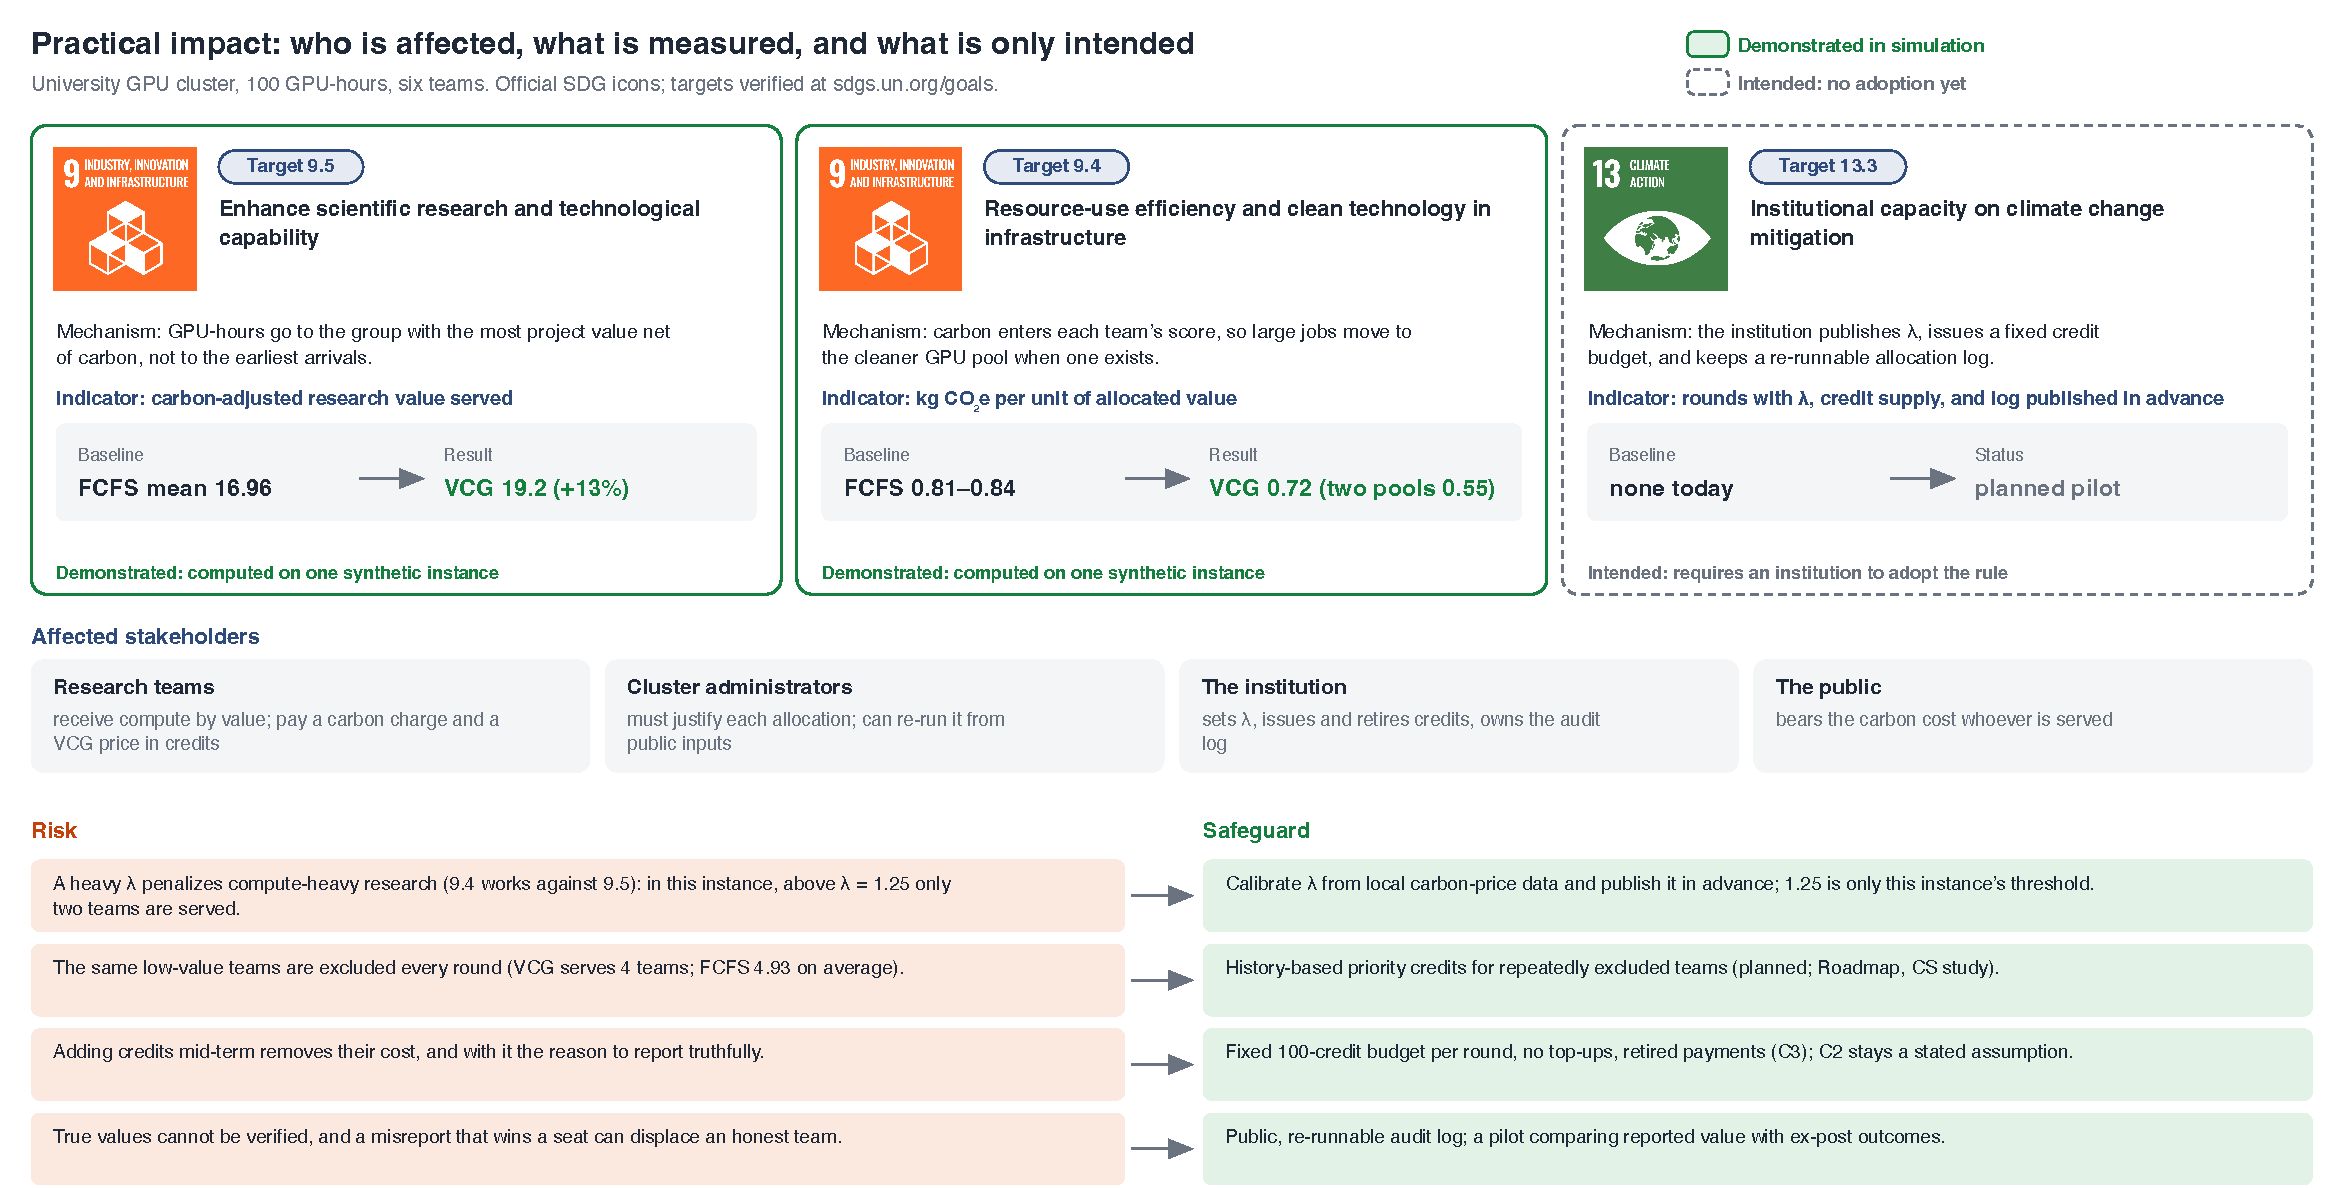
\includegraphics[width=\textwidth]{figures/impact_diagram.pdf}
\caption{Practical-impact diagram with official SDG icons and target codes. Solid green cards are demonstrated only in simulation on one synthetic instance; the dashed card is intended and requires institutional adoption. Each risk is paired with its safeguard.}
\label{fig:impact}
\end{figure*}

\subsubsection*{Future Research Roadmap}
Figure~\ref{fig:roadmap} starts from the limitation that remains after this revision: truthful reporting is verified for one round of one synthetic instance with fixed carbon rates. The \textbf{economics} study (Mustafa Ayub Khan) tests whether fixed-budget credits keep the truth optimal over repeated rounds and how $\lambda$ and the credit supply should be announced; the 2026 prize for microeconomic foundations of stabilisation policy, including the role of announced future policy~\cite{nobel2026}, motivates the second question. The \textbf{computer-science} study (Temur Akhtamjonov, Gihun Lee) adds several GPU types with measured power and grid intensity~\cite{radovanovic2021carbon}, replaces exact search with an integer program checked against it, and tests history-based credits so that the same teams are not excluded every round~\cite{karma2023}. The \textbf{behavioral} study (Gihun Lee) asks players to write a reason before seeing the result, to separate misunderstanding~\cite{li2017} from a preference for winning~\cite{cooperfang2008}. Our duet partners FP8, who offered their simulation benchmark, are a possible collaborator for the first two studies. The earlier milestone table is kept in Appendix~E (Table~\ref{tab:trajectory}).

\begin{figure*}[t]
\centering
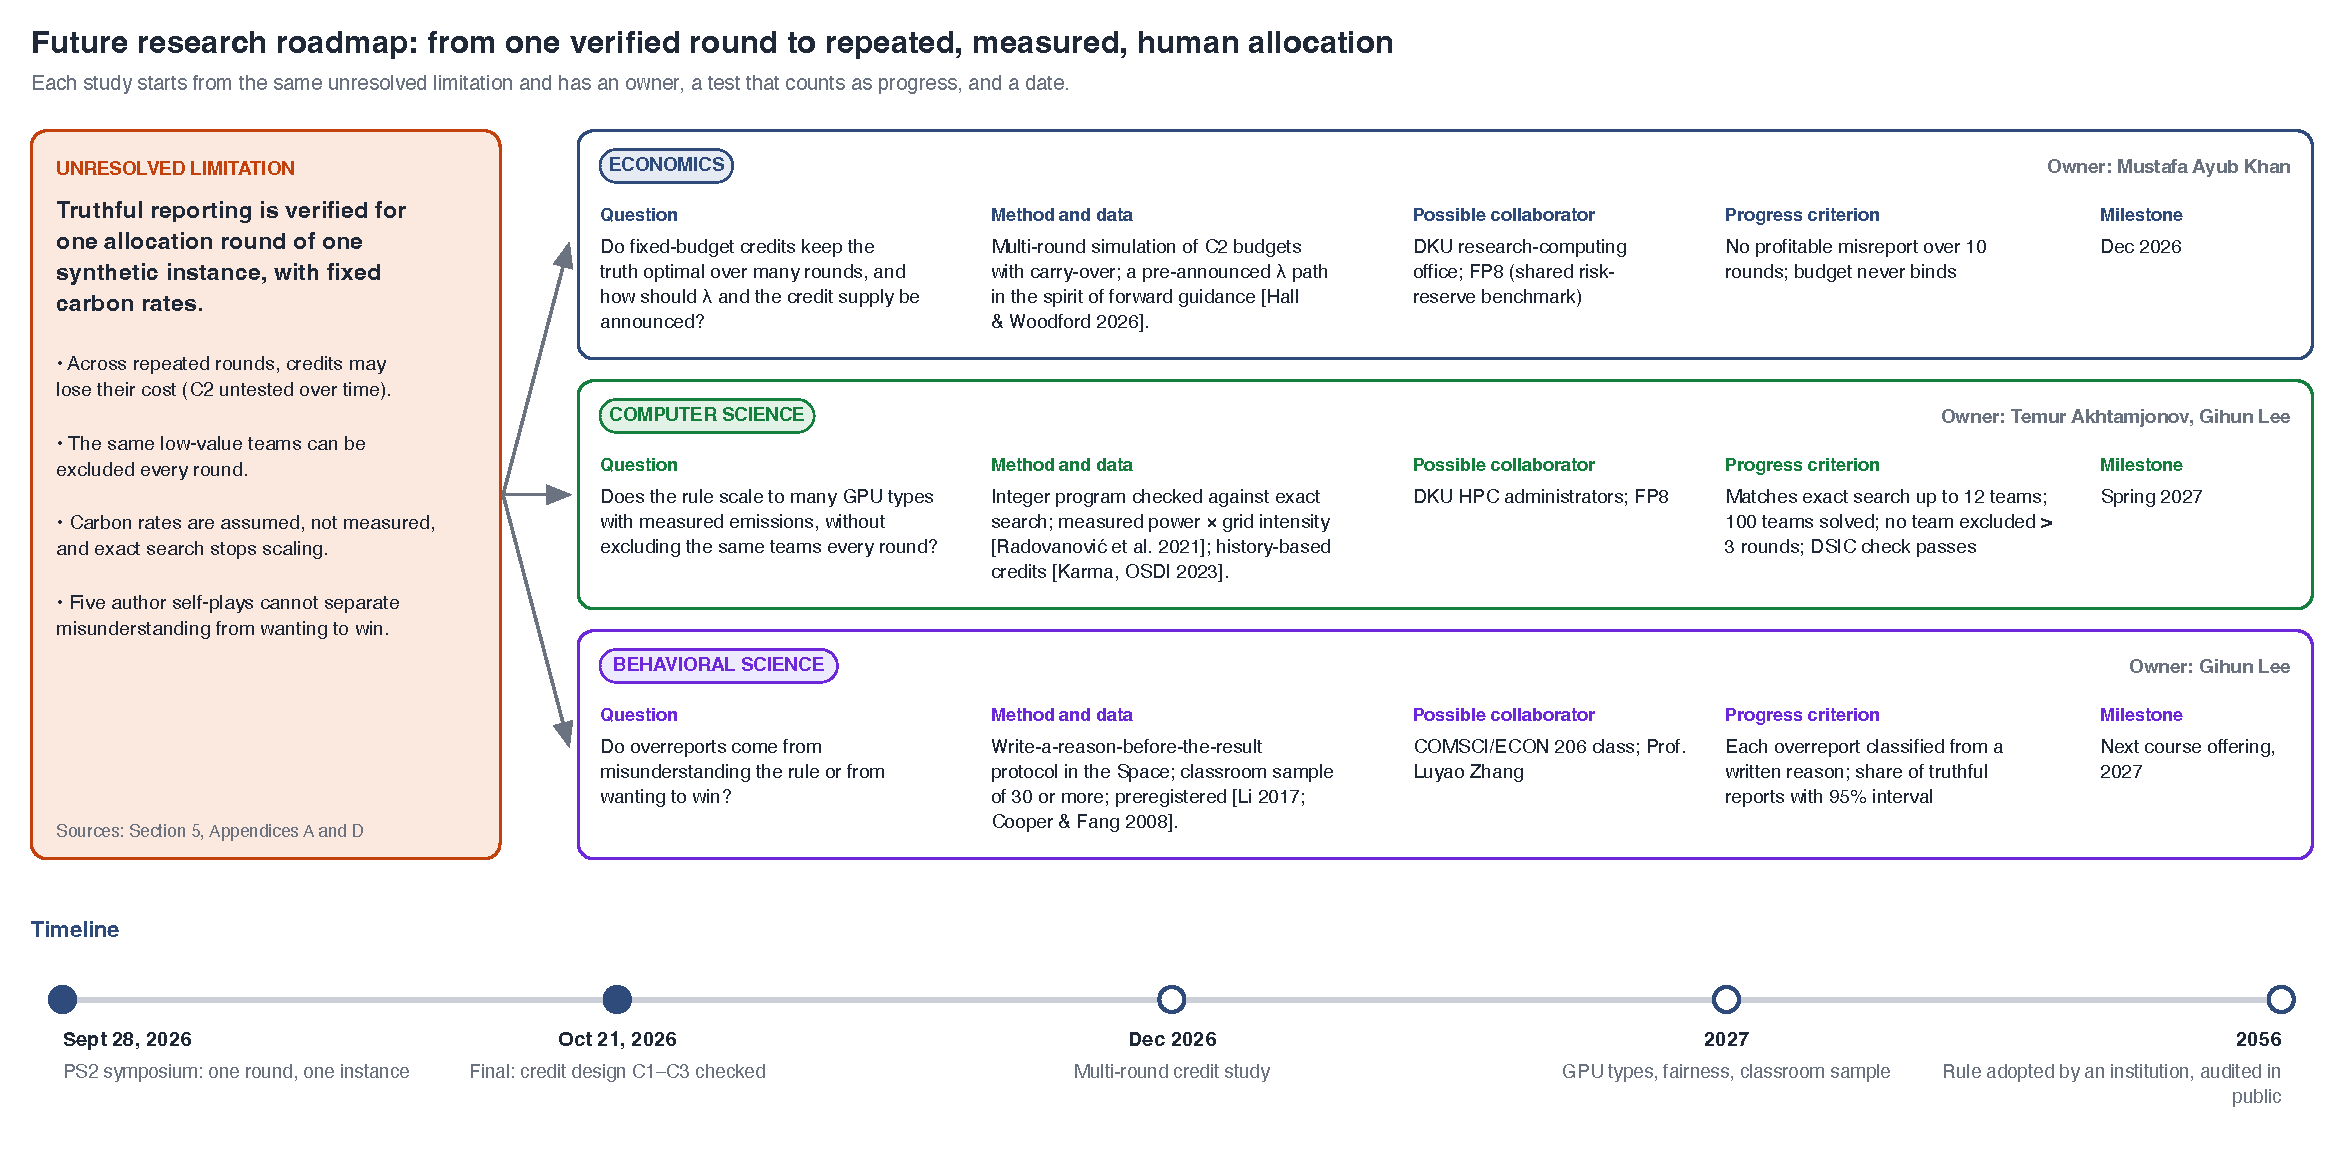
\includegraphics[width=\textwidth]{figures/roadmap_diagram.pdf}
\caption{Future research roadmap. One unresolved limitation feeds an economics, a computer-science, and a behavioral study, each with a question, method and data, possible collaborator, progress criterion, milestone, and owner.}
\label{fig:roadmap}
\end{figure*}

\vspace{3pt}

\noindent
\noindent\textbf{Expected 2056 Nobel Prize and Turing Award contribution statement.}
By 2056, we aim to be recognized for an efficient, publicly auditable governance framework for scarce shared infrastructure, integrating an incentive-compatible mechanism, verifiable computation, and behavioral evidence on truthful reporting. \textbf{Revised after the 2026 prize:} the framework must also include a credible institutional rule for the credit supply and for announcing $\lambda$, because the price that makes truth optimal is only as real as teams expect the credits to be (Appendix~D.6). Progress moves from this six-team simulation to a real institutional pilot, correctable through a public, re-runnable audit log.

\subsubsection*{Open Science Statement}
GitHub (\url{https://github.com/dku-comsci-econ206-Autumn2026/FP05-PS2-Team-A}) contains the FCFS/VCG code, tests, and outputs, including the carbon-weight sweep (\texttt{lambda\_sweep.csv}); a self-contained Colab notebook (\url{https://colab.research.google.com/drive/14eo8a2HWUbbBtv-m-ia4xRiL4V6Iwtun}) that also holds the two-GPU-pool extension; a Hugging Face Space (\url{https://huggingface.co/spaces/dku-comsci-econ206-2026/PS2_Team_A}, commit \texttt{ad5604b}); README with run instructions. Inputs are synthetic ($d_i\in\{15,20,25\}$, $v_i\in\{3,6,9\}$; the Space allows wider ranges), clearly labeled. Review-ready results come from commit \texttt{d93fc2e}; final results from commit \texttt{8a656a4}. Limitation: exact enumeration does not scale past small team counts.

\end{document}
